\chapter{Metodología y Experimentación}

Este capítulo comienza abordando los temas explicados en el marco teórico y su implementación a los datos en este trabajo de tesis. Primero, se muestra en análisis estadístico de los datos, número de variables, cantidad de registros, cantidad de datos faltantes y cantidad de datos atípicos o anómalos; acompañado de descripciones visuales como series de tiempo por estación de cada variable, seguido de matrices de correlación entre estaciones por variable. Después, se menciona cómo se eliminan datos no deseables y se acompletan dichos registros para así, por último, tener una base de datos decente para llevar a cabo la experimentación y obtención de resultados discutidos en el capítulo siguiente.



\section{Análisis Estadístico y Limpieza de la Base de Datos}

Las estaciones de monitoreo indican las tendencias puntuales en la calidad del aire, pero sólo representan microambientes alrededor de ellas, por lo que se utilizan {\em métodos de interpolación espacial} para calcular los niveles de contaminantes en los lugares donde no hay estaciones de monitoreo.

La interpolación es el proceso de predecir valores en sitios sin muestrear. Los métodos de interpolación espacial incorporan información sobre la posición geográfica de los puntos de muestra, de modo que los puntos más cercanos entre sí tienen una mayor correlación y similitud que los que están más lejos. En este trabajo se evalúan los siguientes métodos de interpolación: Diagramas de Voronoi (DV), Distancia Inversa Ponderada (DIP), Funciones de Base Radial (FBR), Kriging Ordinario (KO) y Kriging Universal (KU).

La recolección de los datos se hace a partir del promedio de mediciones por hora. La base de datos cuenta con lo siguiente:\begin{itemize}
\item Trece estaciones de monitoreo.
\item 1,542,696 mediciones del promedio por hora (desde 1993-01-01 00:00:00 hrs. hasta 2018-12-31 23:00:00 hrs.).
\item Mediciones de quince variables por estación.
\end{itemize}
Luego se cuenta el número de datos faltantes en la base de datos por variable. 
\begin{table}[H]
\centering
\caption{Contaminantes y variables que recopilan las estaciones de monitoreo del SIMA con los nombres correspondientes de las variables en el código fuente \citep{sernagit}}
\begin{adjustbox}{max width=0.9\textwidth}
\begin{tabular}{|c|c|r|}
\hline
Variable &Nomenclatura MEEAMM  &Cantidad de \texttt{NaN} \\ \hline
Tiempo & timestamp   & 0              \\ \hline
\begin{tabular}[c]{@{}l@{}}Monóxido de Carbono\end{tabular}  & CO          & 253,474         \\ \hline
Óxido Nítrico    & NO          & 410,737         \\ \hline
\begin{tabular}[c]{@{}l@{}}Bióxido de Nitrógeno\end{tabular}  & NO$_{2}$         & 412,339         \\ \hline
\begin{tabular}[c]{@{}l@{}}Óxidos de Nitrógeno\end{tabular}  & NO$_{X}$         & 413,766         \\ \hline
Ozono  & O$_{3}$          & 305185         \\ \hline
\begin{tabular}[c]{@{}l@{}}Partículas menores a 10 micras\end{tabular}  & PM$_{10}$        & 159,985         \\ \hline
\begin{tabular}[c]{@{}l@{}}Partículas menores a 2.5 micras\end{tabular} & PM$_{2.5}$       & 1,014,253        \\ \hline
\begin{tabular}[c]{@{}l@{}}Presión Barométrica\end{tabular}  & pressure    & 610,362         \\ \hline
\begin{tabular}[c]{@{}l@{}}Precipitación Pluvial\end{tabular} & rainfall    & 489,331         \\ \hline
\begin{tabular}[c]{@{}l@{}}Humedad Relativa\end{tabular}  & humidity    & 550,968         \\ \hline
\begin{tabular}[c]{@{}l@{}}Bióxido de Azufre\end{tabular}  & SO$_{2}$         & 343,180         \\ \hline
Radiación Solar  & solar       & 675,701         \\ \hline
\begin{tabular}[c]{@{}l@{}}Temperatura Ambiental\end{tabular} & temperature & 109,143         \\ \hline
\begin{tabular}[c]{@{}l@{}}Velocidad del Viento\end{tabular} & velocity    & 109,590         \\ \hline
\begin{tabular}[c]{@{}l@{}}Dirección del Viento\end{tabular} & direction   & 178,126         \\ \hline
Total    &     & 7,554,588      \\  \hline
\end{tabular}
\end{adjustbox}
\end{table}


\begin{figure}[H]
\centering
\subfigure[Cantidad de datos conocidos y datos desconocidos por variable] {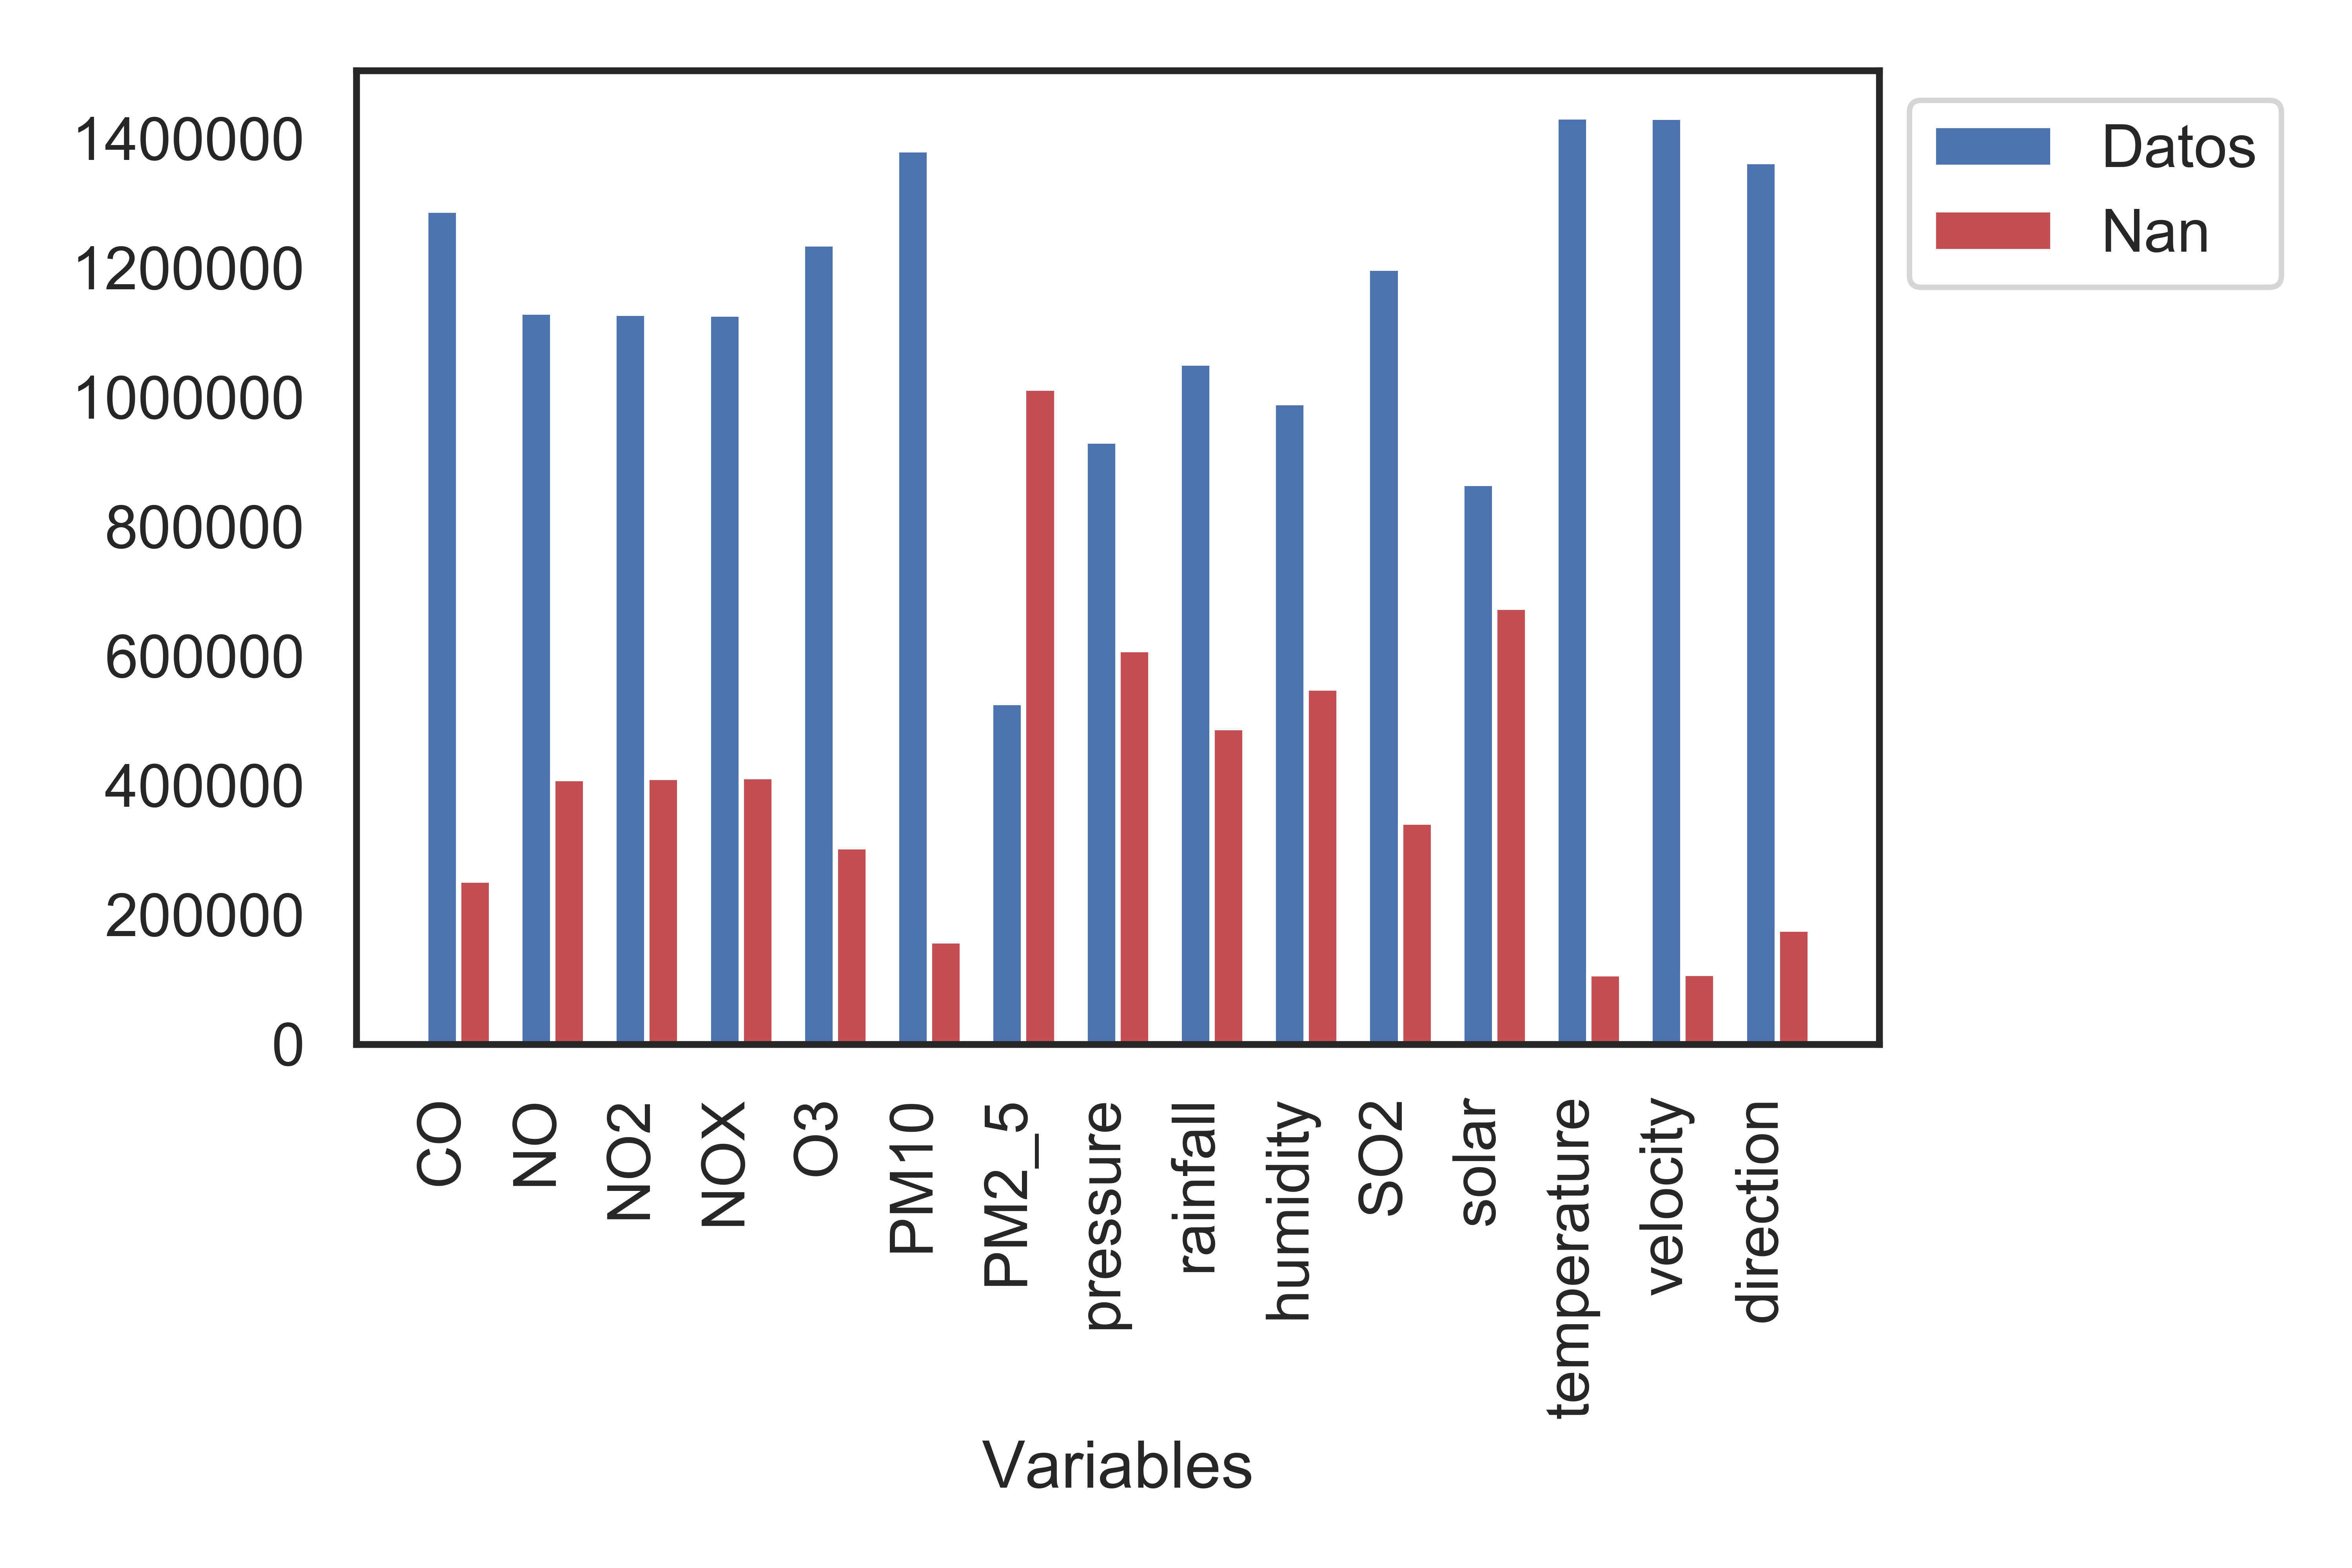
\includegraphics[width=72.5mm]{./BarPlot_All_2}}
\subfigure[Porcentaje de datos conocidos y datos desconocidos por variable]{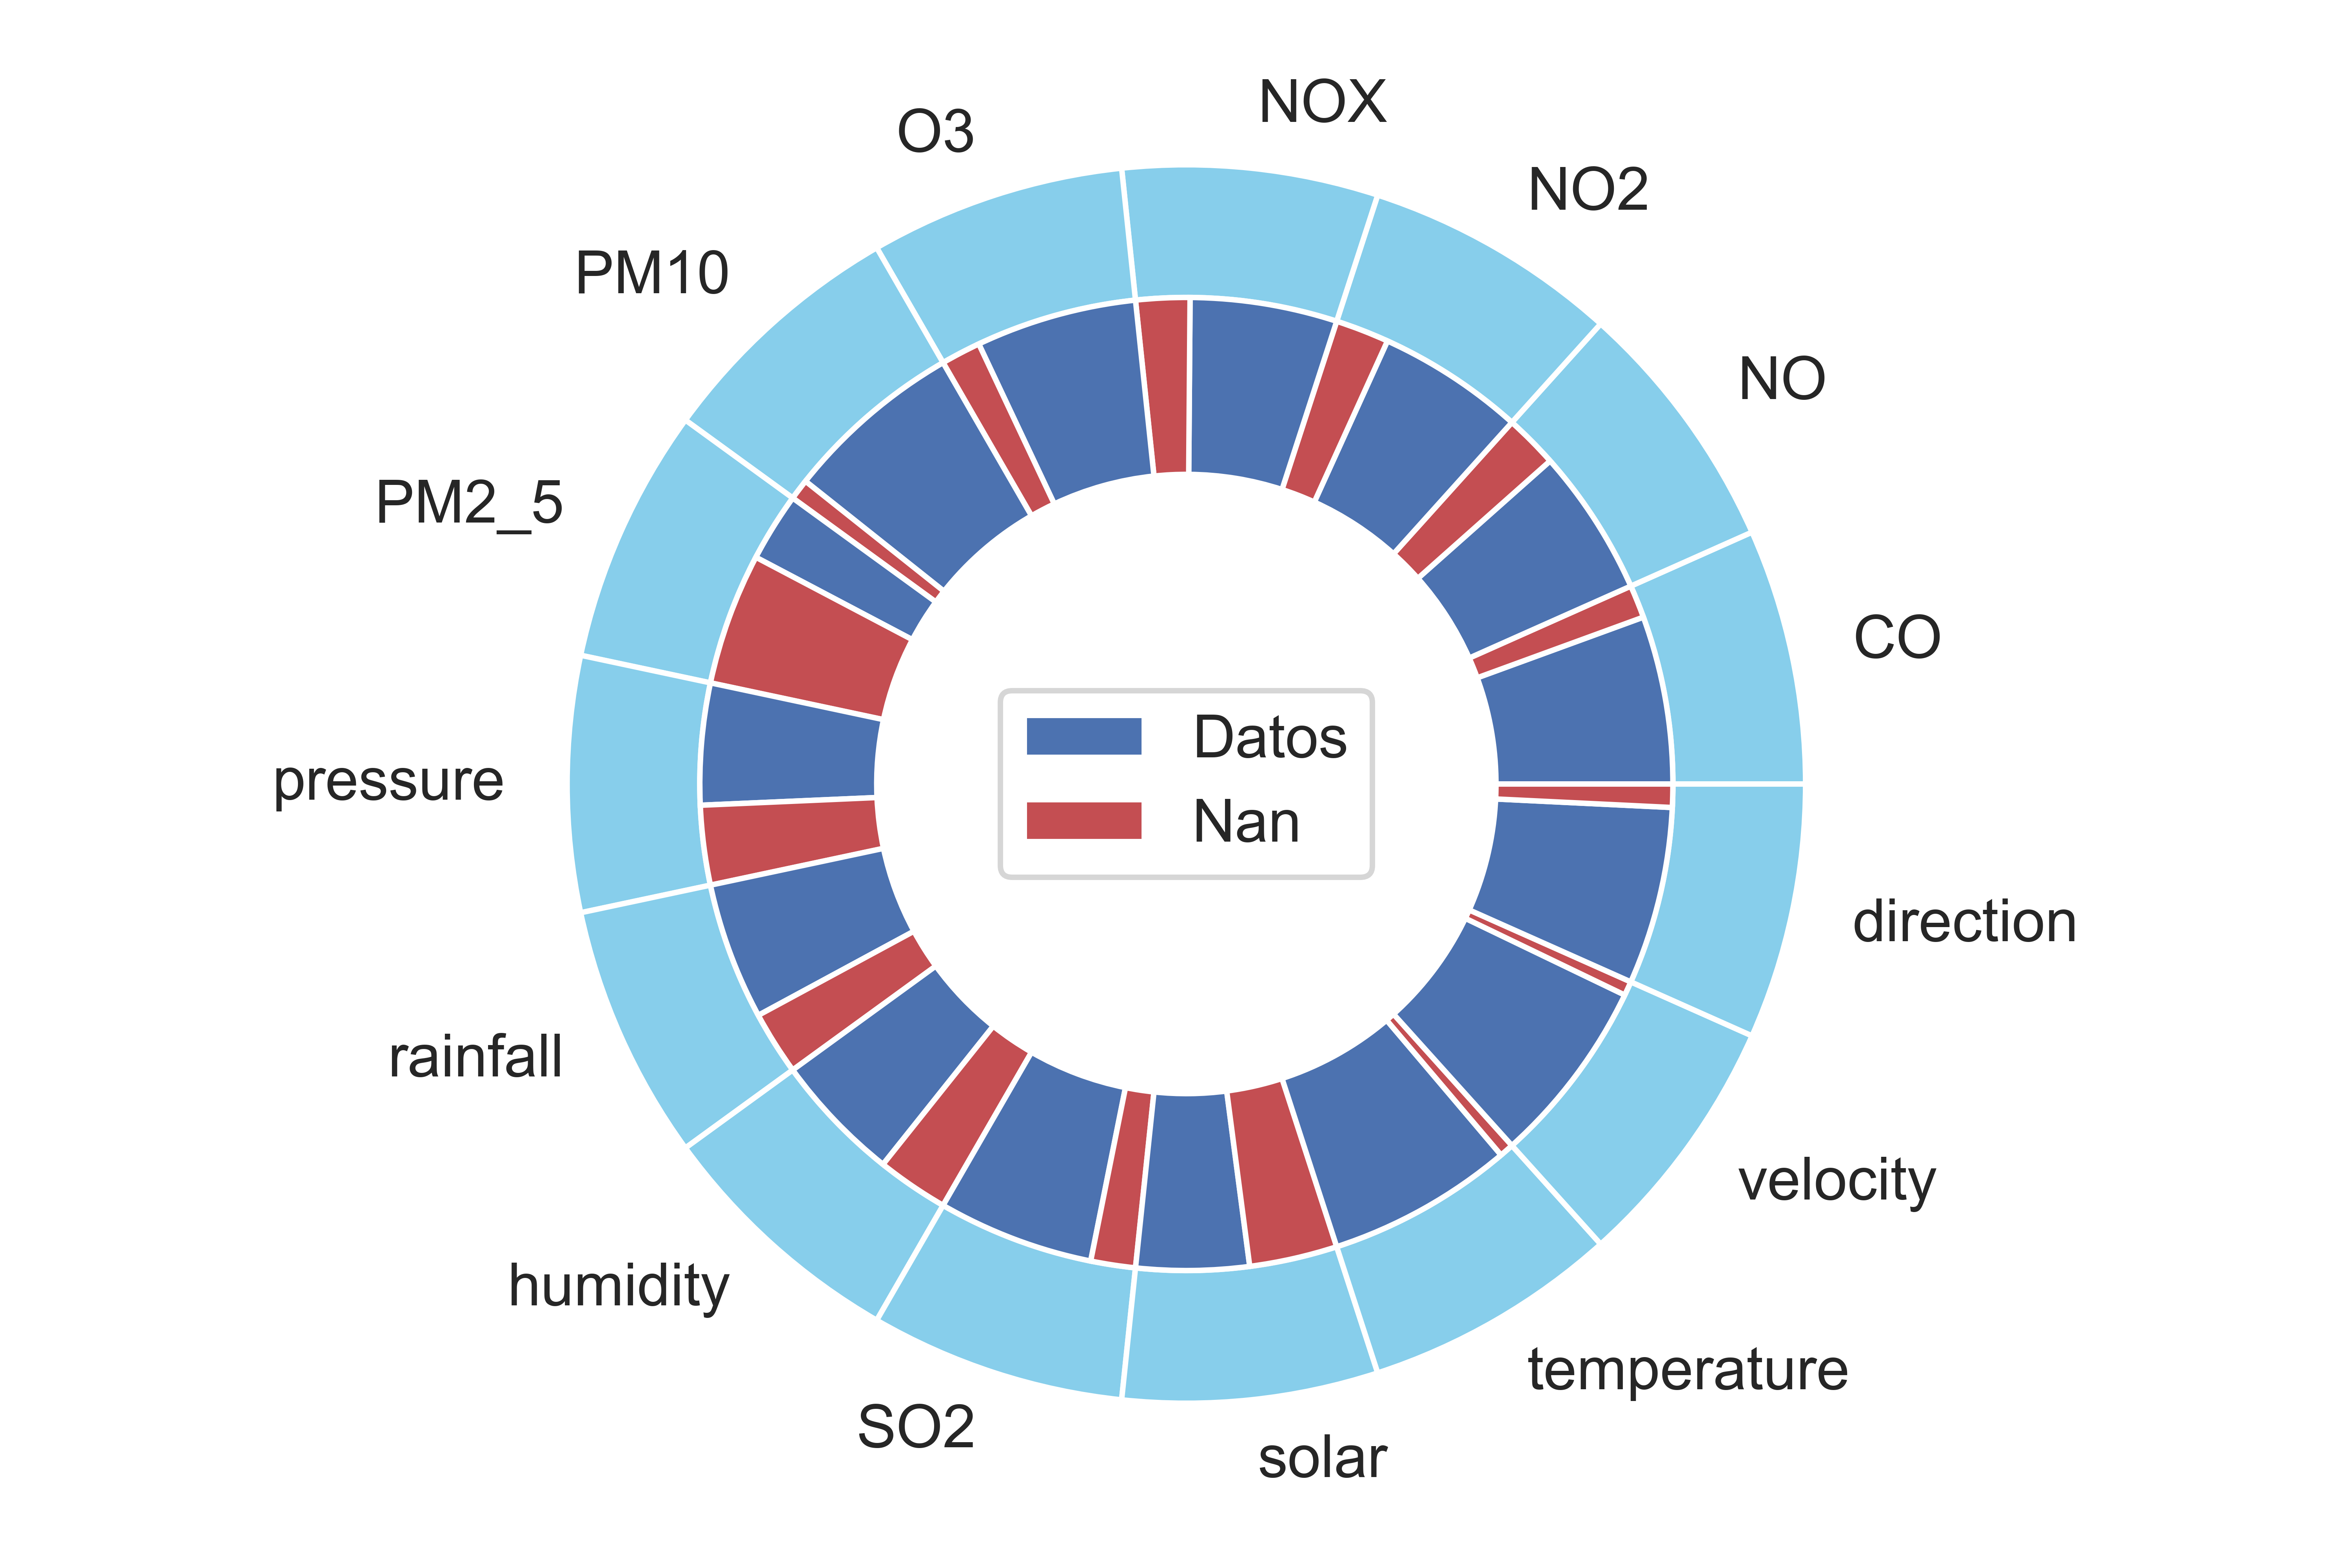
\includegraphics[width=72.5mm]{./BarPie}}
\subfigure[Porcentaje de datos conocidos y datos desconocidos por variable]{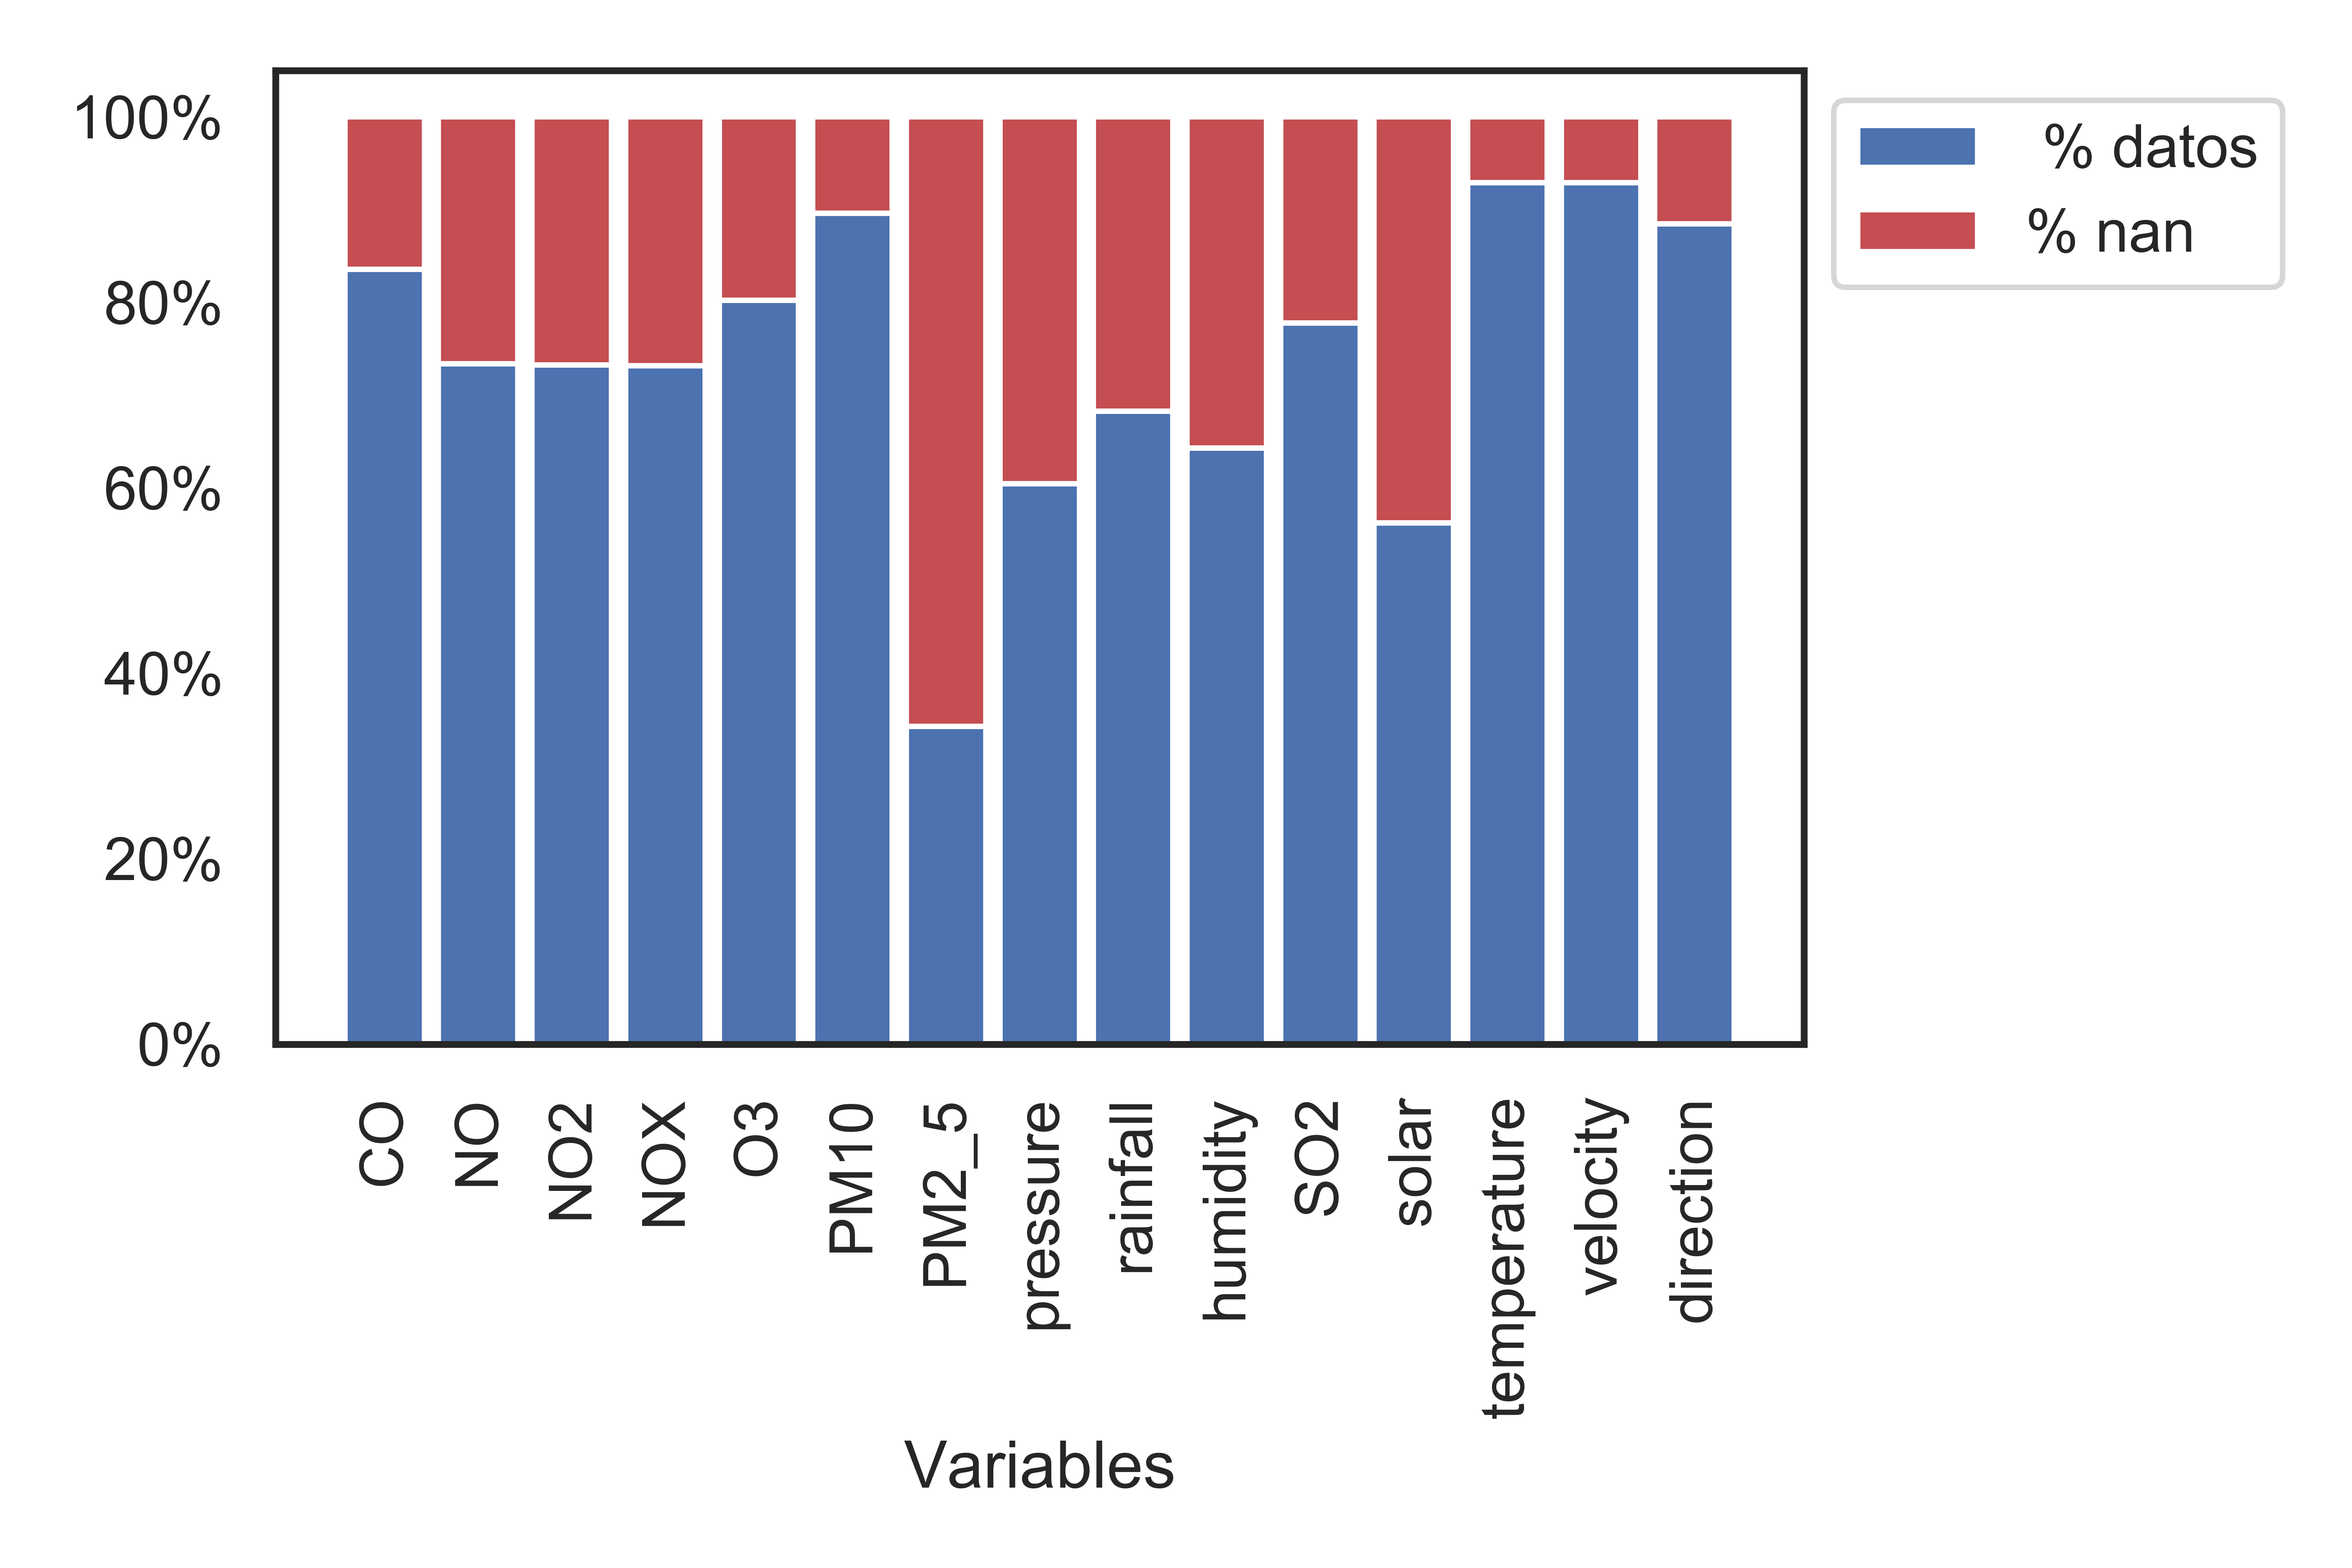
\includegraphics[width=72.5mm]{./BarPlot_All}}
\subfigure[Porcentaje de datos conocidos y datos desconocidos]{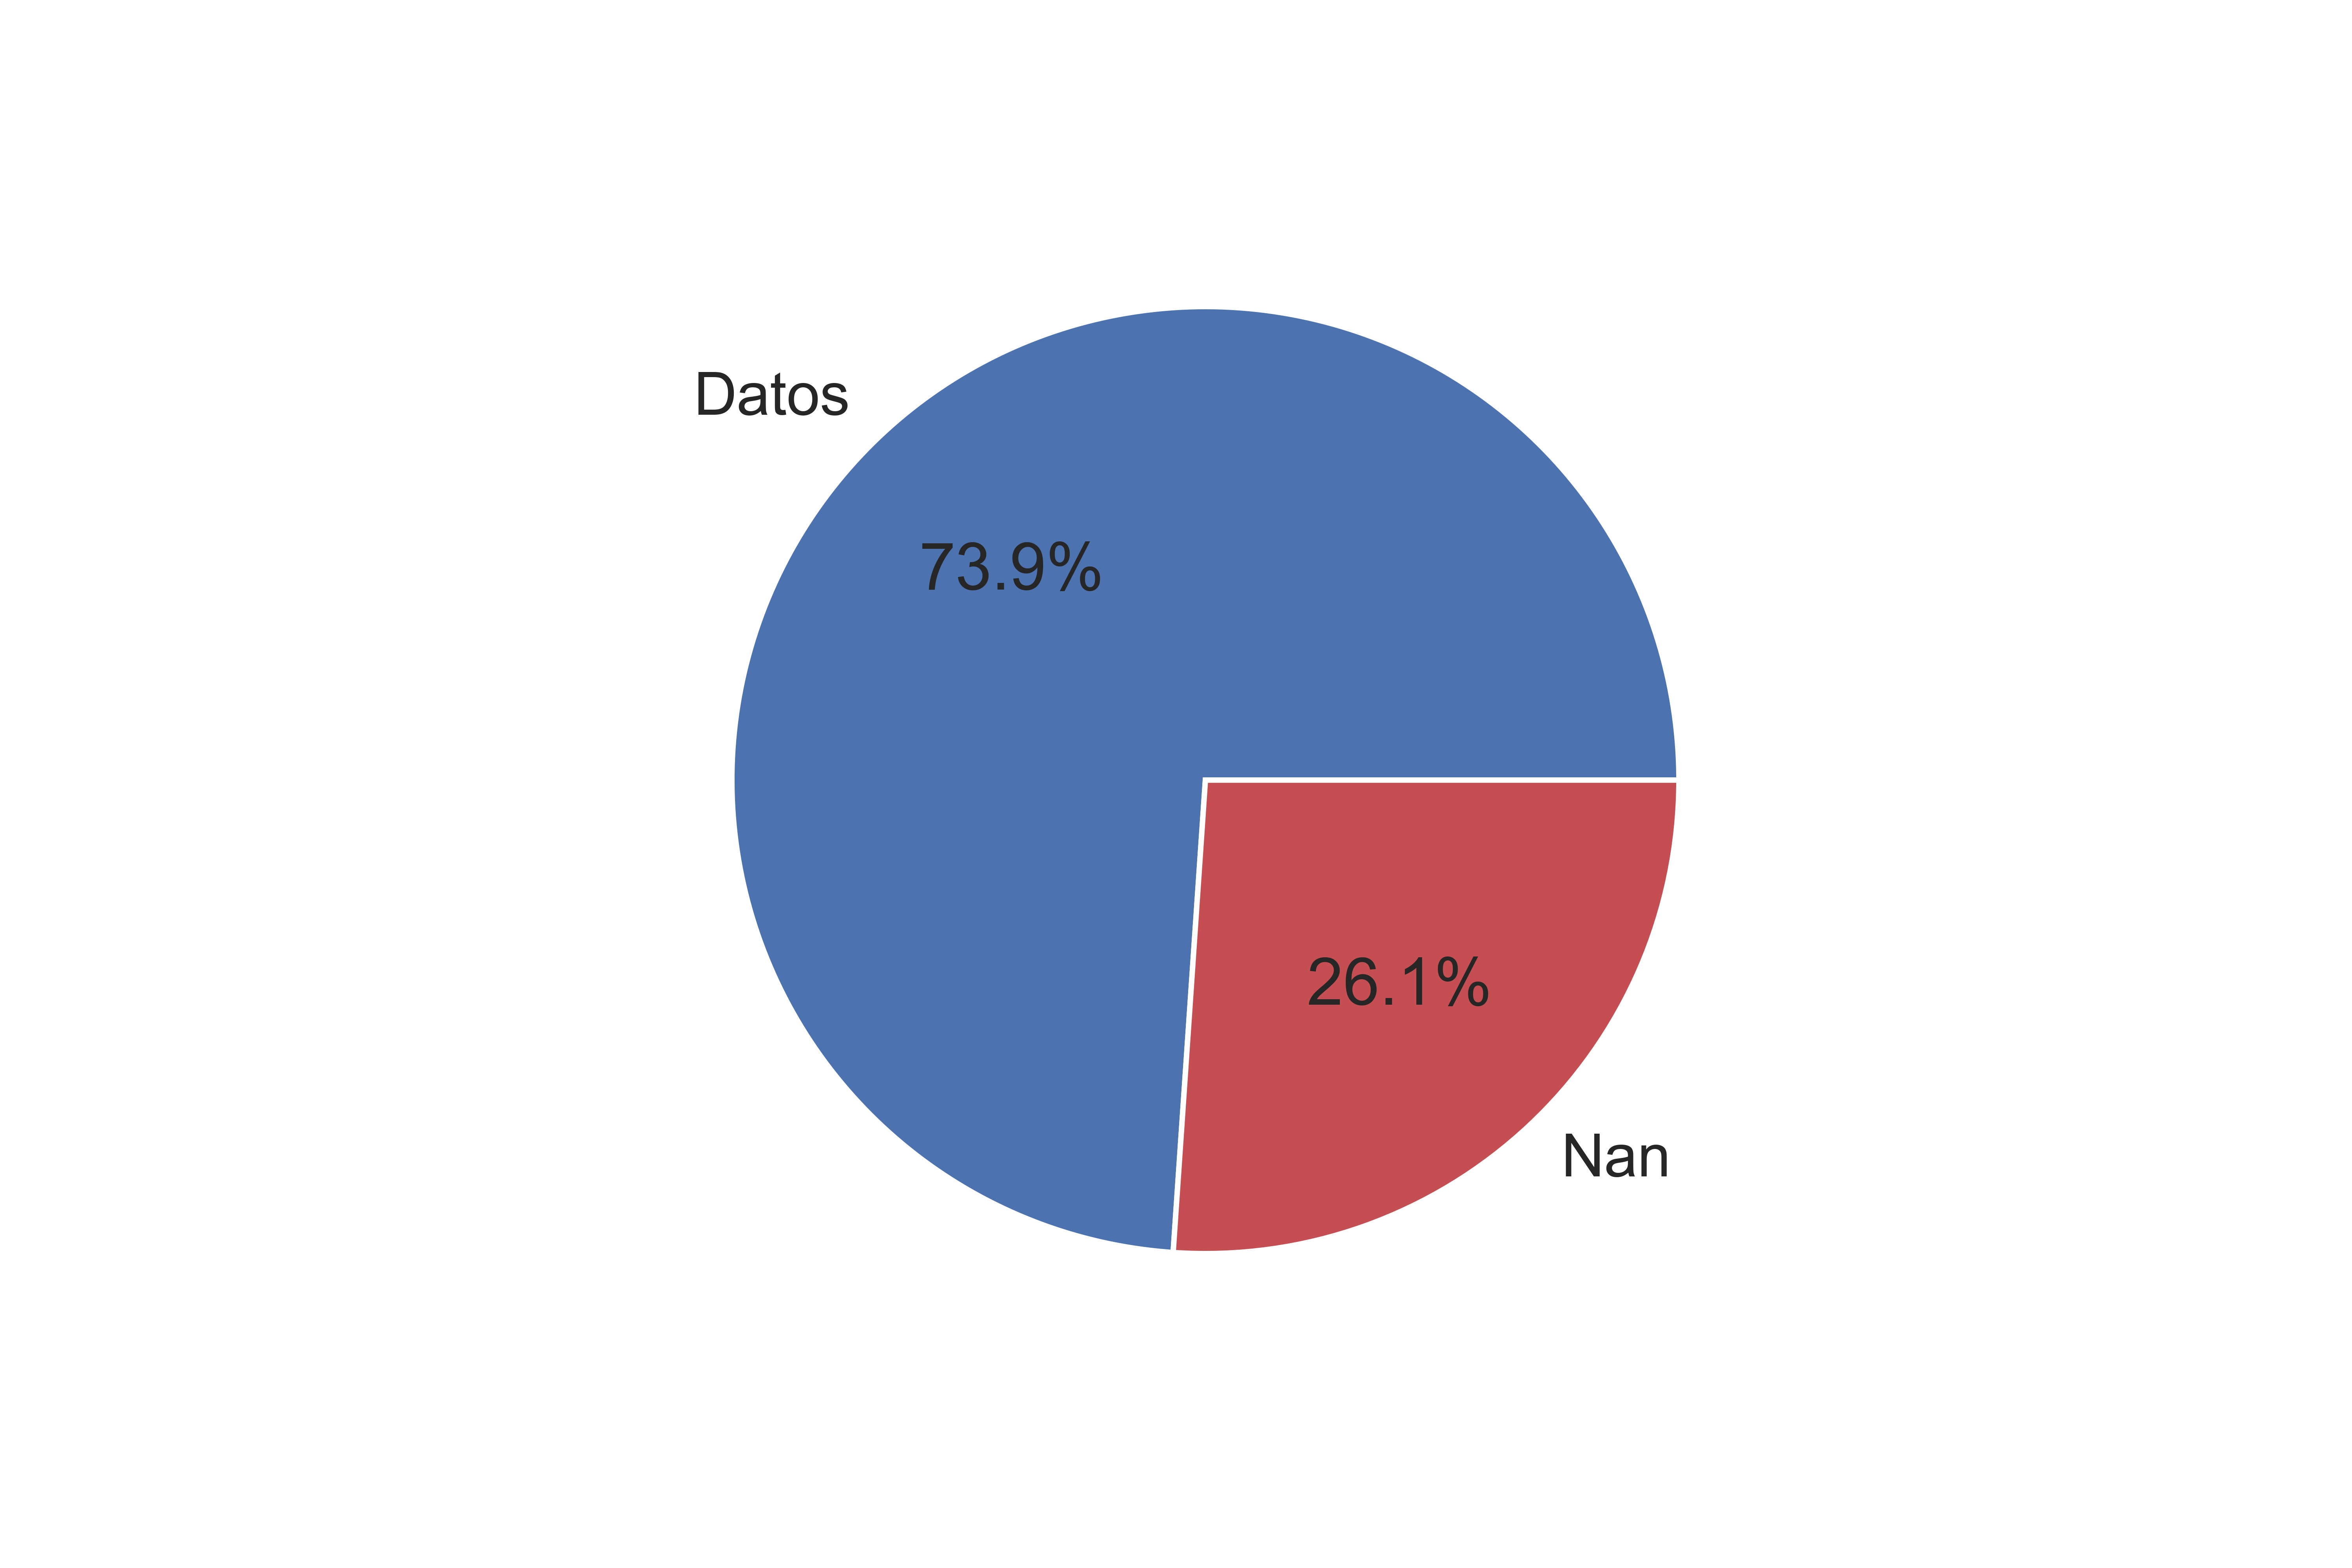
\includegraphics[width=72.5mm]{./BarPie_2}}
\caption{Datos conocidos y desconocidos (NaN) registrados por SIMA}
\label{figure1}
\end{figure}

De las quince variables con las que cuenta SIMA, que son: CO, NO, NO$_{2}$, NO$_{X}$, O$_{3}$, PM$_{10}$, PM$_{2.5}$, {\em Presión atmosférica, Precipitación pluvial, Humedad relativa}, SO$_{2}$, {\em Radiación solar, Temperatura ambiental, Velocidad del viento} y \textit{Dirección del viento}; se analizan cada una por individual. Lo primero que se hace es seleccionar los datos desde el año 2016, ya que algunas estaciones fueron puestas a trabajar hasta el año 2017; para recopilar la información de las variables en estas estaciones se hace el promedio de las estaciones más cercanas sin valores registrados para, posteriormente asignárselos.

Después de identificar la cantidad de datos faltantes, se prosigue con los valores que no son faltantes pero son no permitidos por estar fuera del rango de medición, esto es, el valor existe, aunque el valor de la medición fue provocado por una falla en el sensor de la estación de monitoreo. Los valores mínimos y máximos para cada variable se muestran en la tabla \ref{permitidos}. 

\begin{table}[H]
\centering
\caption{Valores fuera de rango por falla en analizadores y sensores de los diferentes parámetros en las estaciones de monitoreo atmosférico}
\begin{adjustbox}{max width=0.9\textwidth}
\begin{tabular}{|c|c|c|}
\hline
Parámetro &\multicolumn{2}{|c|}{Valores no permitidos}  \\ \hline
 &Menor a la lectura &Mayor a la lectura    \\ \hline
Partículas menores a 10 micras &2 &850\\
Partículas menores a 2.5 micras &2 &850\\
Ozono &1 &200\\   
Óxido Nítrico &1 &350\\ 
Bióxido de Nitrógeno &1 &150\\
Oxídos de Nitrógeno &1 &350\\
Bióxido de Azufre &1 &200\\
Monóxido de Carbono &0.05 &15\\
Temperatura ambiental &-15 &50\\
Precipitación pluvial &0 &---\\
Humedad relativa &0 &100 \\
Presión barométrica &650 &750 \\
Radiación solar &0 &1.2 \\
Velocidad del ciento &0 &60 \\
Dirección del viento &0 &360\\ \hline
\end{tabular}
\end{adjustbox}
\label{permitidos}
\end{table}

Después de identificar los valores faltantes y los valores no permitidos, se eliminan de la base de datos. Para completar los registros eliminados lo que se hace es interpolar los datos mediante la función \texttt{interpolate} con el método \texttt{time} cuando el valor fue un valor no permitido,  ya que la función \texttt{interpolate} consiste en seleccionar los valores al tiempo $t-1$ y al tiempo $t+1$ para asignar un valor en el registro al tiempo $t$ mediante una interpolación lineal. Para el caso de las estaciones en las que no se cuenta con información al tiempo $t-1$ y $t+1$, pues no se encontraban en operación la estación, lo que se hace es calcular el promedio por variable de las estaciones más cercanas a la estación que aún no está en operación, asignándole el valor promedio calculado hora a hora.


\subsection{Monóxido de Carbono (CO)} 
\begin{figure}[H]
\centering
\subfigure[Serie de tiempo de CO original] {\includegraphics[width=7cm, height=15cm]{./Serie_Nans_CO}}
\subfigure[Serie de tiempo de CO rellenando datos desconocidos]{\includegraphics[width=7cm, height=15cm]{./Serie_CO}}
\caption{Series de tiempo de CO desde 2016 hasta 2018}
\label{serieCO}
\end{figure}

La variable CO presenta datos faltantes durante intervalos de tiempo en los tres años seleccionados (ver figura \ref{serieCO} (a)), tales valores se completan haciendo el promedio de las estaciones cercanas a la estación con los datos faltantes  y se asigna el valor promedio a ésta, se puede apreciar en la figura \ref{serieCO} (b) que ya todas la estaciones cuentan con los valores en los tres años seleccionados, además se puede apreciar que la serie de tiempo es estacionaria, pues parece variar en torno a una media fija.

\begin{figure}[H]
\centering
\subfigure[Histograma de CO por estación] {\includegraphics[width=15cm, height=10cm]{./Histogram__2_CO_3}}
\subfigure[Histograma de CO]{\includegraphics[width=12cm, height=5cm]{./Histogram__2_CO_2}}
\caption{Histogramas de CO}
\label{histCO}
\end{figure}

La figura \ref{serieCO} muestra los gráficos de series de tiempo para la variable CO por estación y la figura \ref{histCO} muestra los histogramas de los datos por estación de la variable CO. De la figura \ref{serieCO} se puede observar que si bien las trece series de tiempo muestran características muy similares, es decir, son parecidas en estacionariedad en el tiempo, los histogramas de la figura \ref{histCO} son diferentes entre algunas estaciones, ya que el histograma resume los datos a través de la dimensión del tiempo, y al hacerlo, se pierden las características clave de los datos que dependen del tiempo.

\begin{figure}[H]
\centering
\includegraphics[width=12cm, height=10cm]{./Corr_CO_CO}
\caption{Matriz de correlación de CO entre estaciones}
\label{corrCOCO}
\end{figure}

La figura \ref{corrCOCO} muestra que la variable CO se correlaciona positivamente alto (correlaciones mayores a 0.2) entre la mayoría de las estaciones, pues la estación Sureste 2 muestra correlaciones bajas (correlaciones menores a 0.2) contra las estaciones Noroeste, Sur y Sureste 3.

\begin{figure}[H]
\centering
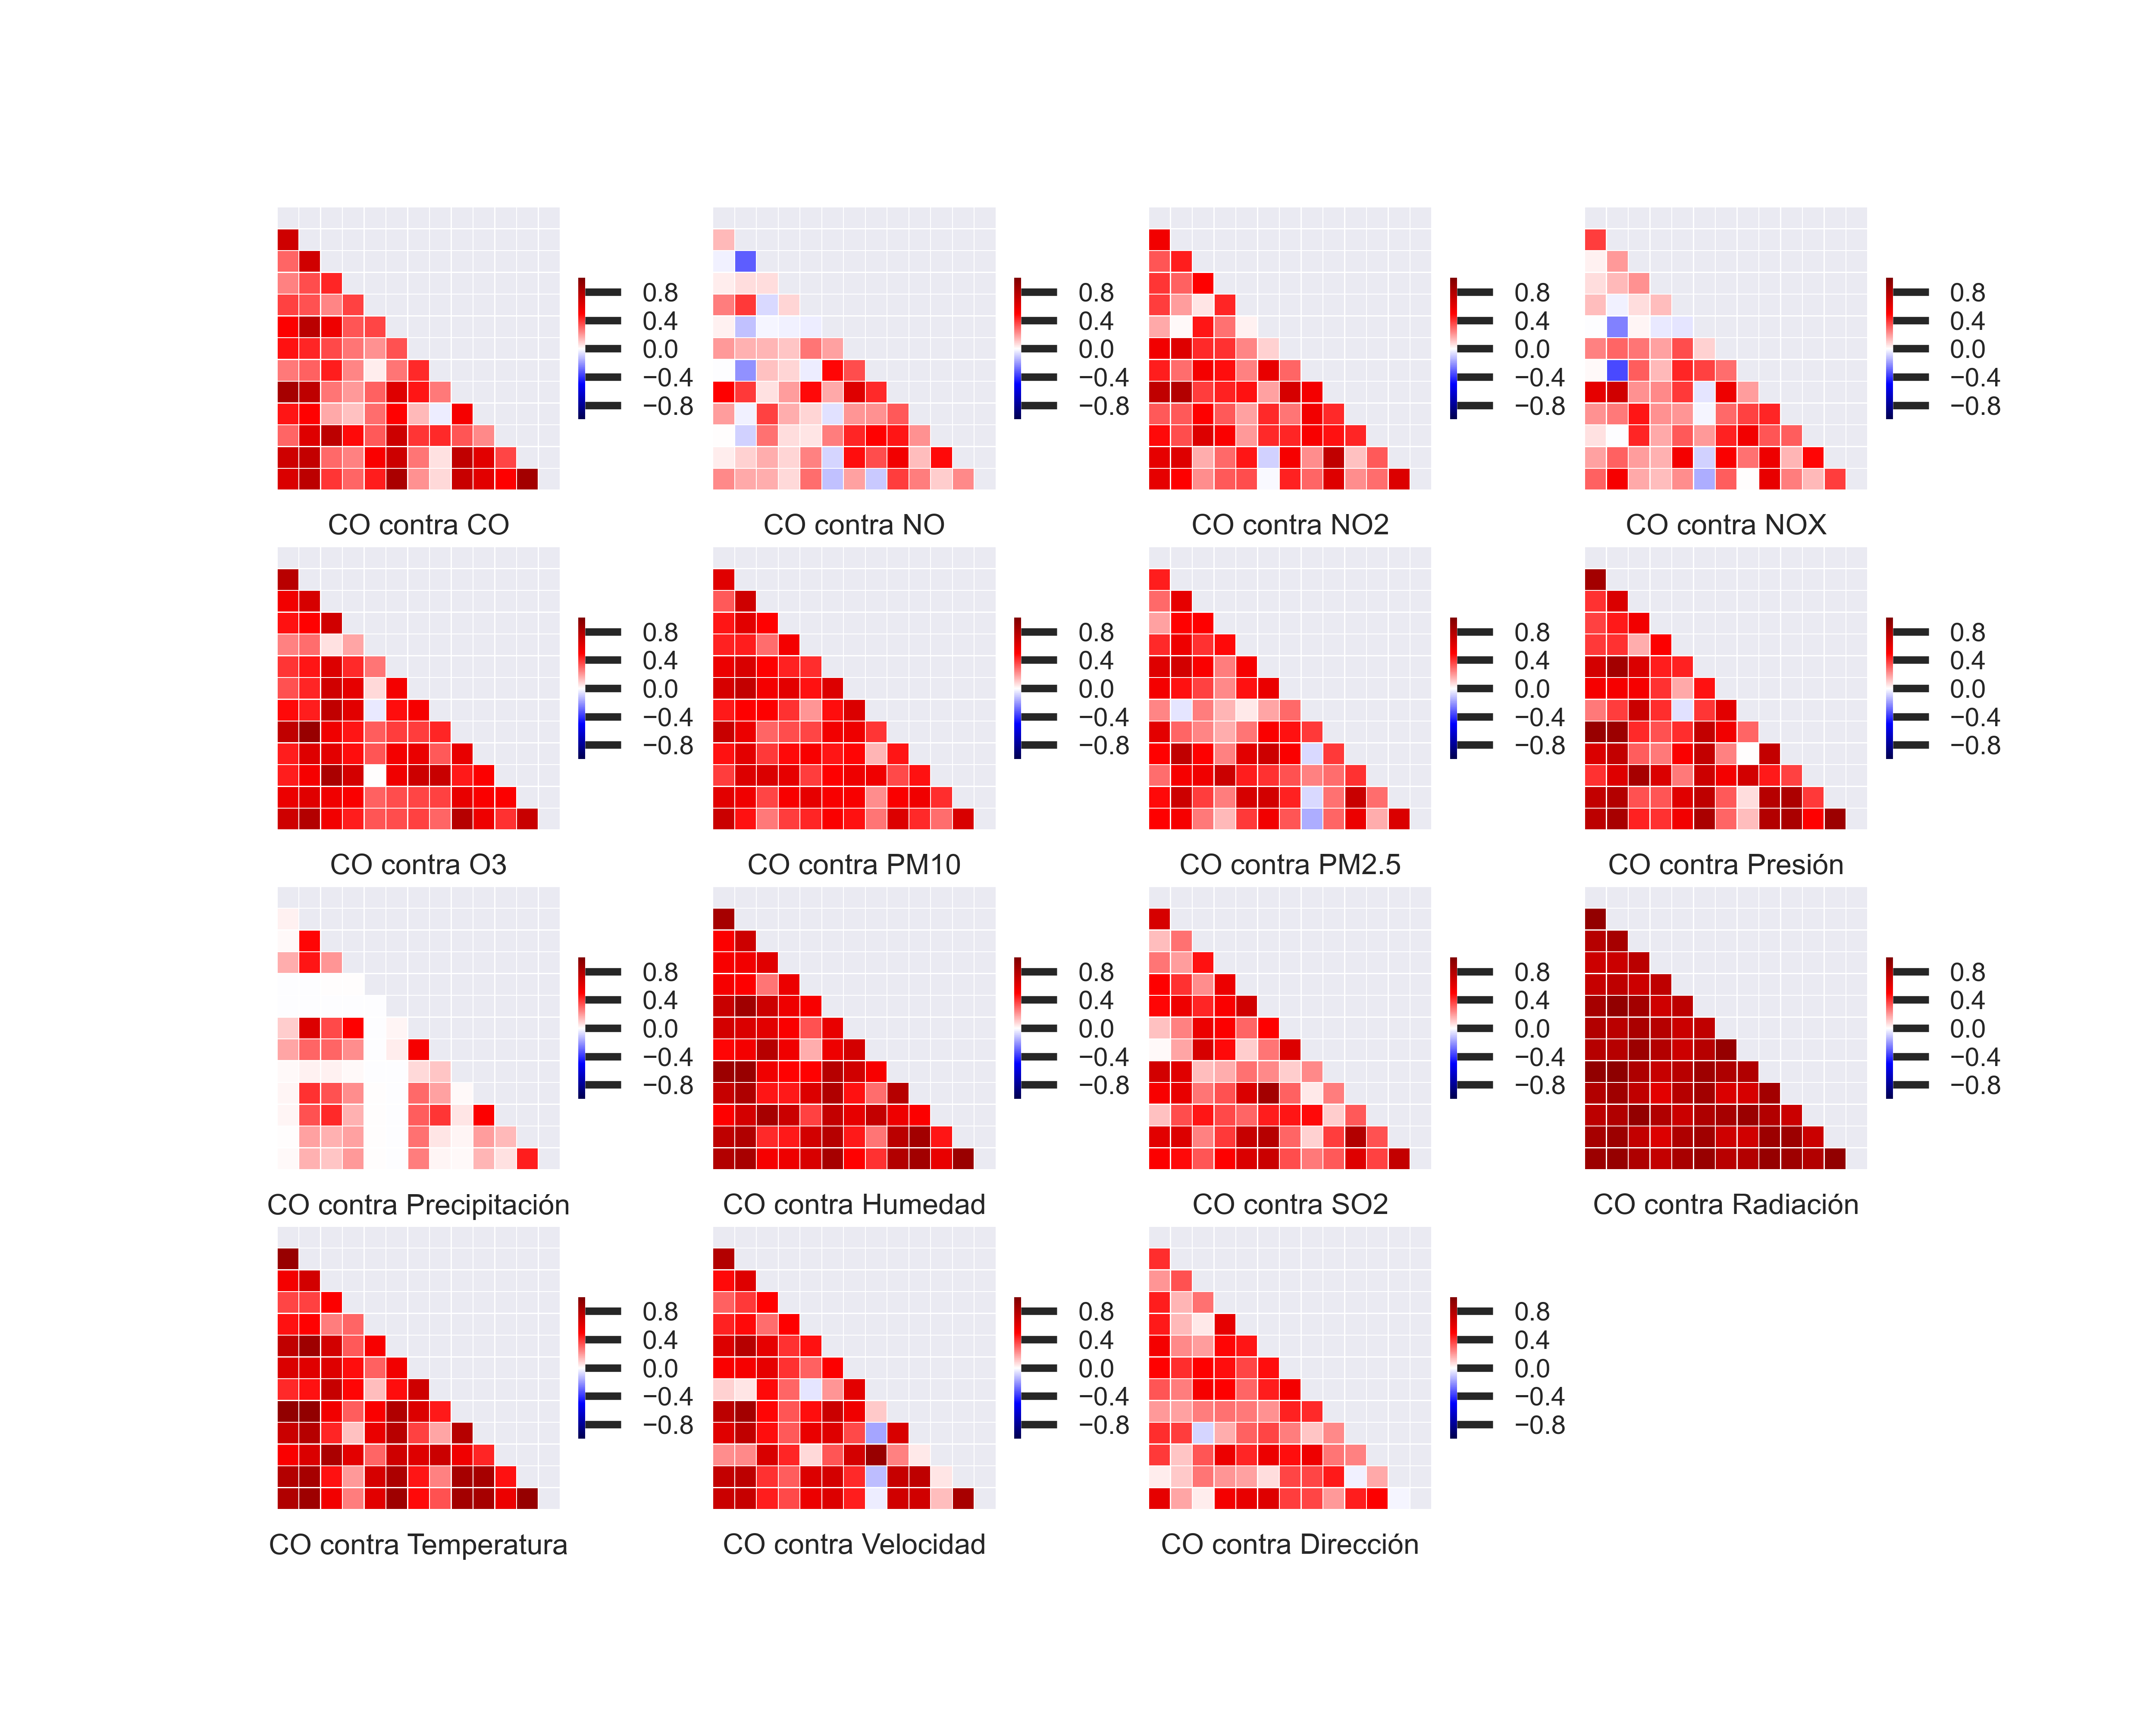
\includegraphics[width=15cm, height=13cm]{./Corr_CO_all_final}
\caption{Matriz de correlación de CO contra el resto de las variables}
\label{corrCO}
\end{figure}


La correlaciones de la variable CO con el resto de las variables se correlaciona positivamente mostrando correlaciones mayores a 0.2 (ver figura \ref{corrCO}), sin embargo para la variable {\em precipitación pluvial} las correlaciones son menores a 0.2 (ver figura \ref{corrCO}).






\subsection{Óxido Nítrico (NO)}
\begin{figure}[H]
\centering
\subfigure[Serie de tiempo de NO original] {\includegraphics[width=7cm, height=15cm]{./Serie_Nans_NO}}
\subfigure[Serie de tiempo de NO rellenando datos desconocidos]{\includegraphics[width=7cm, height=15cm]{./Serie_NO}}
\caption{Series de tiempo de NO desde 2016 hasta 2018}
\label{serieNO}
\end{figure}

La variable NO además de tener datos faltantes que se rellenan haciendo el promedio de las estaciones cercanas y asignando el promedio a las estaciones sin registros, se puede apreciar en la figura \ref{serieNO} que la serie de tiempo es estacionaria pues parece variar entorno a una media fija.

\begin{figure}[H]
\centering
\subfigure[Histograma de NO por estación] {\includegraphics[width=15cm, height=10cm]{./Histogram__3_NO_3}}
\subfigure[Histograma de NO]{\includegraphics[width=12cm, height=5cm]{./Histogram__3_NO_2}}
\caption{Histogramas de NO}
\label{histNO}
\end{figure}

La figura \ref{serieNO} muestra los gráficos de series de tiempo para la variable NO por estación y la figura \ref{histNO} muestra un histograma de los datos por estación de la variable NO. De la figura \ref{serieNO} se puede observar que si bien las trece series de tiempo muestran características muy similares, los histogramas de la figura \ref{histNO} son diferentes, ya que el histograma resume los datos a través de la dimensión del tiempo, y al hacerlo, se pierden las características clave de los datos que dependen del tiempo.

\begin{figure}[H]
\centering
\includegraphics[width=12cm, height=10cm]{./Corr_NO_NO}
\caption{Matriz de correlación de NO entre estaciones }
\label{corrNONO}
\end{figure}

La figura \ref{corrNONO} muestra que la variable NO se correlaciona positivamente alto (correlaciones mayores a 0.2) entre la mayoría de las estaciones, ya que las estaciones Centro y Sureste 2 muestran correlaciones menores a 0.2 contra el resto de la estaciones. Además para las estaciones Noroeste, Noreste y Norte muestran correlaciones bajas.

\begin{figure}[H]
\centering
\includegraphics[width=15cm, height=13cm]{./Corr_NO_all_final}
\caption{Matriz de correlación de NO contra el resto de las variables}
\label{corrNO}
\end{figure}


Para las correlaciones de la variable {\em precipitación pluvial} y NO$_{X}$, (ver figura \ref{corrNO}) se presentan en algunas estaciones correlaciones altas y correlaciones nulas. Además, para las correlaciones con la variable NO$_{2}$ presenta correlaciones positivas pequeñas para la estación Suroeste 2.





\subsection{Bióxido de Nitrógeno (NO$_{2}$)}
\begin{figure}[H]
\centering
\subfigure[Serie de tiempo de NO$_{2}$ original] {\includegraphics[width=7cm, height=15cm]{./Serie_Nans_NO2}}
\subfigure[Serie de tiempo de NO$_{2}$ rellenando datos desconocidos]{\includegraphics[width=7cm, height=15cm]{./Serie_NO2}}
\caption{Series de tiempo de NO$_{2}$ desde 2016 hasta 2018}
\label{serieNO2}
\end{figure}

La variable NO$_{2}$ presenta datos faltantes durante periodos de tiempo en los tres años que se rellenan haciendo el promedio de las estaciones cercanas, este promedio se le asigna a las estaciones sin registros. También, se puede apreciar en la figura \ref{serieNO2} (b), que la serie de tiempo es estacionaria, ya que parece variar entorno a una media, presentando altas variaciones en el mes de julio del 2017 en las trece estaciones.

\begin{figure}[H]
\centering
\subfigure[Histograma de NO$_{2}$ por estación] {\includegraphics[width=15cm, height=10cm]{./Histogram__4_NO2_3}}
\subfigure[Histograma de NO$_{2}$]{\includegraphics[width=12cm, height=5cm]{./Histogram__4_NO2_2}}
\caption{Histogramas de NO$_{2}$}
\label{histNO2}
\end{figure}

La figura \ref{serieNO2} muestra los gráficos de series de tiempo para la variable NO$_{2}$ por estación y la figura \ref{histNO2} muestra los histogramas de los datos por estación de la variable NO$_{2}$. En la figura \ref{serieNO2} se puede observar que si bien las trece series de tiempo muestran características muy similares, también,  los histogramas de la figura \ref{histNO2} son muy similares a excepción de las estaciones Norte 2 y Sur.

\begin{figure}[H]
\centering
\includegraphics[width=12cm, height=10cm]{./Corr_NO2_NO2}
\caption{Matriz de correlación de NO$_{2}$ entre estaciones }
\label{corrNO2NO2}
\end{figure}

La figura \ref{corrNO2NO2} muestra que la variable NO$_{2}$ se correlaciona positivamente entre la mayoria de las estaciones, ya que la estación Suroeste 2 muestra correlaciones bajas contra las estaciones Noroeste 2, Norte 2 y Suroeste.

\begin{figure}[H]
\centering
\includegraphics[width=15cm, height=13cm]{./Corr_NO2_all_final}
\caption{Matriz de correlación de NO$_{2}$ contra el resto de las variables}
\label{corrNO2}
\end{figure}

La estación Suroeste 2 presenta correlaciones positivas pequeñas contra la variable NO$_{X}$ (ver figura \ref{corrNO2}). Para las correlaciones de la variable {\em precipitación pluvial} se presentan en algunas estaciones correlaciones altas y correlaciones cercanas a cero (ver figura \ref{corrNO2}).






\subsection{Óxidos de Nitrógeno (NO$_{X}$)}
\begin{figure}[H]
\centering
\subfigure[Serie de tiempo de NO$_{X}$ original] {\includegraphics[width=7cm, height=15cm]{./Serie_Nans_NOX}}
\subfigure[Serie de tiempo de NO$_{X}$ rellenando datos desconocidos]{\includegraphics[width=7cm,height=15cm]{./Serie_NOX}}
\caption{Series de tiempo de NO$_{X}$ desde 2016 hasta 2018}
\label{serieNOX}
\end{figure}

La variable NO$_{X}$ además de tener datos faltantes que se rellenan haciendo el promedio de las estaciones cercanas y asignando el promedio a las estaciones sin registros, se puede apreciar en la figura \ref{serieNOX} que la serie de tiempo es estacionaria ya que parece variar en torno a una media fija.

\begin{figure}[H]
\centering
\subfigure[Histograma de NO$_{X}$ por estación] {\includegraphics[width=15cm, height=10cm]{./Histogram__5_NOX_3}}
\subfigure[Histograma de NO$_{X}$]{\includegraphics[width=12cm, height=5cm]{./Histogram__5_NOX_2}}
\caption{Histogramas de NO$_{X}$}
\label{histNOX}
\end{figure}

La figura \ref{serieNOX} muestra los gráficos de series de tiempo para la variable NO$_{X}$ por estación y la figura \ref{histNOX} muestra un histograma de los datos por estación de la variable NO$_{X}$. De la figura \ref{serieNOX} se puede apreciar que en las trece series de tiempo muestran características muy similares, sin embargo, los histogramas de la figura \ref{histNOX} son diferentes, ya que el histograma resume los datos a través de la dimensión del tiempo, y al hacer esto, se pierden las características importantes de los datos que dependen del tiempo.

\begin{figure}[H]
\centering
\includegraphics[width=12cm, height=10cm]{./Corr_NOX_NOX}
\caption{Matriz de correlación de NO$_{X}$ entre estaciones }
\label{corrNOXNOX}
\end{figure}

La correlación de la variable NO$_{X}$ entre estaciones (NO$_{X}$ vs NO$_{X}$) presenta correlaciones positivas pequeñas (ver figura \ref{corrNOXNOX}).  

\begin{figure}[H]
\centering
\includegraphics[width=15cm, height=13cm]{./Corr_NOX_all_final}
\caption{Matriz de correlación de NO$_{X}$  contra el resto de las variables}
\label{corrNOX}
\end{figure}

Las correlaciones de la variable {\em precipitación pluvial}  (ver Figura \ref{corrNOX}) muestran que para algunas correlaciones entre estaciones se presentan corelaciones positivas bajas.





\subsection{Ozono (O$_{3}$)}
\begin{figure}[H]
\centering
\subfigure[Serie de tiempo de O$_{3}$ original] {\includegraphics[width=7cm, height=15cm]{./Serie_Nans_O3}}
\subfigure[Serie de tiempo de O$_{3}$ rellenando datos desconocidos]{\includegraphics[width=7cm,height=15cm]{./Serie_O3}}
\caption{Series de tiempo de O$_{3}$ desde 2016 hasta 2018}
\label{serieO3}
\end{figure}

La variable O$_{3}$ además de tener datos faltantes que se completan haciendo el promedio de las estaciones cercanas y asignando el promedio a las estaciones sin registros, se puede apreciar en la figura \ref{serieO3} que la serie de tiempo es estacionaria pues varía entorno a un valor.

\begin{figure}[H]
\centering
\subfigure[Histograma de O$_{3}$ por estación] {\includegraphics[width=15cm, height=10cm]{./Histogram__6_O3_3}}
\subfigure[Histograma de O$_{3}$]{\includegraphics[width=12cm, height=5cm]{./Histogram__6_O3_2}}
\caption{Histogramas de O$_{3}$}
\label{histO3}
\end{figure}

La figura \ref{serieO3} muestra los gráficos de series de tiempo para la variable O$_{3}$ por estación y la figura \ref{histO3} muestra un histograma de los datos por estación de la variable O$_{3}$. De la figura \ref{serieO3} se puede observar que si bien las trece series de tiempo muestran características similares, los histogramas de la figura \ref{histO3} son distintos, pues el histograma resume los datos a través de la dimensión del tiempo, y al hacerlo, se pierden las características principales de los datos que dependen del tiempo.

\begin{figure}[H]
\centering
\includegraphics[width=12cm, height=10cm]{./Corr_O3_O3}
\caption{Matriz de correlación de O$_{3}$ entre estaciones }
\label{corrO32}
\end{figure}

La figura \ref{corrO32} muestra que la variable O$_{3}$ se correlaciona positivamente alto en todas las estaciones ya que la mayor correlación es de 0.99 entre las estaciones Noroeste 2 y Sur, mientras que la menor correlación encontrada es de 0.57 entre las estaciones Suroeste 2 y Sureste 2.

\begin{figure}[H]
\centering
\includegraphics[width=15cm, height=13cm]{./Corr_O3_all_final}
\caption{Matriz de correlación de O$_{3}$ contra el resto de las variables}
\label{corrO3}
\end{figure}

Para las correlaciones de la variable {\em precipitación pluvial} se presentan en algunas estaciones correlaciones altas y correlaciones cercanas a cero (ver figura \ref{corrO3}), para el resto de las variables la variable O$_{3}$ se correlaciona positivamente alto en todas las estaciones.





\subsection{Partículas Menores a 10 Micras (PM$_{10}$)}
\begin{figure}[H]
\centering
\subfigure[Serie de tiempo de PM$_{10}$ original] {\includegraphics[width=7cm, height=15cm]{./Serie_Nans_PM10}}
\subfigure[Serie de tiempo de PM$_{10}$ rellenando datos desconocidos]{\includegraphics[width=7cm,height=15cm]{./Serie_PM10}}
\caption{Series de tiempo de PM$_{10}$ desde 2016 hasta 2018}
\label{seriePM10}
\end{figure}

La variable PM$_{10}$ además de tener datos faltantes que se completan haciendo el promedio de las estaciones cercanas y luego se asigna el promedio a las estaciones sin datos, se puede apreciar en la figura \ref{seriePM10} que la serie de tiempo es estacionaria pues varía entorno a una media.

\begin{figure}[H]
\centering
\subfigure[Histograma de PM$_{10}$ por estación] {\includegraphics[width=15cm, height=10cm]{./Histogram__7_PM10_3}}
\subfigure[Histograma de PM$_{10}$]{\includegraphics[width=12cm, height=5cm]{./Histogram__7_PM10_2}}
\caption{Histogramas de PM$_{10}$}
\label{histPM10}
\end{figure}

La figura \ref{seriePM10} muestra los gráficos de series de tiempo para la variable PM$_{10}$ por estación y la figura \ref{histPM10} muestra un histograma de los datos por estación de la variable PM$_{10}$. De la figura \ref{seriePM10} se puede observar que las trece series de tiempo muestran características similares, pero, los histogramas de la figura \ref{histPM10} son diferentes, pues el histograma resume los datos a través de la dimensión del tiempo, y al hacer esto, se pierden las características principales de los datos que dependen del tiempo.

\begin{figure}[H]
\centering
\includegraphics[width=12cm, height=10cm]{./Corr_PM10_PM10}
\caption{Matriz de correlación de PM$_{10}$ entre estaciones }
\label{corrPM10_2}
\end{figure}

La figura \ref{corrPM10_2} muestra que la variable PM$_{10}$ se correlaciona positivamente alto entre todas las estaciones ya que la mayor correlación es de 0.73 entre las estaciones Norte 2 y Noreste, mientras que la menor correlación encontrada es de 0.20 entre las estaciones Noreste 2 y Noroeste 2.

\begin{figure}[H]
\centering
\includegraphics[width=15cm, height=13cm]{./Corr_PM10_all_final}
\caption{Matriz de correlación de PM$_{10}$ contra el resto de las variables}
\label{corrPM10}
\end{figure}


Para las correlaciones de la variable {\em precipitación pluvial} se presentan algunas estaciones con correlaciones altas y correlaciones cercanas a cero (ver figura \ref{corrPM10}), para el resto de las variables la variable PM$_{10}$ se correlaciona positivamente alto en todas las estaciones.





\subsection{Partículas Menores a 2.5 Micras (PM$_{2.5}$)}
\begin{figure}[H]
\centering
\subfigure[Serie de tiempo de PM$_{2.5}$ original] {\includegraphics[width=7cm, height=15cm]{./Serie_Nans_PM2_5}}
\subfigure[Serie de tiempo de PM$_{2.5}$ rellenando datos desconocidos]{\includegraphics[width=7cm,height=15cm]{./Serie_PM2_5}}
\caption{Series de tiempo de PM$_{2.5}$ desde 2016 hasta 2018}
\label{seriePM2_5}
\end{figure}

La variable PM$_{2.5}$ además de tener datos faltantes que se rellenan haciendo el promedio de las estaciones cercanas y asignando el promedio a las estaciones sin registros, se puede apreciar en la figura \ref{seriePM2_5} que la serie de tiempo es estacionaria ya que parece variar en torno a una media fija.

\begin{figure}[H]
\centering
\subfigure[Histograma de PM$_{2.5}$ por estación] {\includegraphics[width=15cm, height=10cm]{./Histogram__8_PM2_5_3}}
\subfigure[Histograma de PM$_{2.5}$]{\includegraphics[width=12cm, height=5cm]{./Histogram__8_PM2_5_2}}
\caption{Histogramas de PM$_{2.5}$}
\label{histPM2_5}
\end{figure}

La figura \ref{seriePM2_5} muestra los gráficos de series de tiempo para la variable PM$_{2.5}$ por estación y la figura \ref{histPM2_5} muestra un histograma de los datos por estación de la variable PM$_{2.5}$. De la figura \ref{seriePM2_5} se puede observar que si bien las trece series de tiempo muestran características muy similares, los histogramas de la figura \ref{histPM2_5} son diferentes, ya que el histograma resume los datos a través de la dimensión del tiempo, y al hacerlo, se pierden las características clave de los datos que dependen del tiempo.

\begin{figure}[H]
\centering
\includegraphics[width=12cm, height=10cm]{./Corr_PM2_5_PM2_5}
\caption{Matriz de correlación de PM$_{2.5}$ entre estaciones }
\label{corrPM25_2}
\end{figure}

La figura \ref{corrPM25_2} muestra que la variable PM$_{2.5}$ se correlaciona positivamente alto entre todas las estaciones ya que la mayor correlación es de 0.97 entre las estaciones Norte y Sur, mientras que la menor correlación encontrada es de 0.28 entre las estaciones Sur y Noroeste.

\begin{figure}[H]
\centering
\includegraphics[width=15cm, height=13cm]{./Corr_PM2_5_all_final}
\caption{Matriz de correlación de PM$_{2.5}$ contra el resto de las variables}
\label{corrPM2_5}
\end{figure}


Para las correlaciones de la variable {\em precipitación pluvial} se presentan en algunas estaciones correlaciones altas y correlaciones cercanas a cero (ver figura \ref{corrPM2_5}), para el resto de las variables la variable PM$_{2.5}$ se correlaciona positivamente alto en todas las estaciones.




\subsection{Presión Barométrica}
\begin{figure}[H]
\centering
\subfigure[Serie de tiempo de {\em presión barométrica} original] {\includegraphics[width=7cm, height=15cm]{./Serie_Nans_pressure}}
\subfigure[Serie de tiempo de {\em presión barométrica} rellenando datos desconocidos]{\includegraphics[width=7cm,height=15cm]{./Serie_pressure}}
\caption{Series de tiempo de {\em presión barométrica} desde 2016 hasta 2018}
\label{seriePressure}
\end{figure}

La variable {\em presión barométrica} además de tener datos faltantes que se rellenan haciendo el promedio de las estaciones cercanas y asignando el promedio a las estaciones sin registros, se puede apreciar en la figura \ref{seriePressure} que la serie de tiempo es estacionaria ya que parece variar entorno a una media.

\begin{figure}[H]
\centering
\subfigure[Histograma de {\em presión barométrica} por estación] {\includegraphics[width=15cm, height=10cm]{./Histogram__9_Pressure_3}}
\subfigure[Histograma de {\em presión barométrica}]{\includegraphics[width=12cm, height=5cm]{./Histogram__9_Pressure_2}}
\caption{Histogramas de {\em presión barométrica}}
\label{histPressure}
\end{figure}

La figura \ref{seriePressure} muestra los gráficos de series de tiempo para la variable {\em presión barométrica} por estación y la figura \ref{histPressure} muestra un histograma de los datos por estación de la variable {\em presión barométrica}. De la figura \ref{seriePressure} se puede observar que si bien las trece series de tiempo muestran características muy similares, los histogramas de la figura \ref{histPressure} son diferentes, ya que el histograma resume los datos a través de la dimensión del tiempo, y al hacerlo, se pierden las características más importantes de los datos que dependen del tiempo.

\begin{figure}[H]
\centering
\includegraphics[width=12cm, height=10cm]{./Corr_pressure_pressure}
\caption{Matriz de correlación de {\em presión barométrica} entre estaciones }
\label{corrpressure2}
\end{figure}

La figura \ref{corrpressure2} muestra que la variable {\em presión barométrica} se correlaciona positivamente alto entre la mayoría de las estaciones ya que la estación Sureste 3 presenta dos correlaciones positivas bajas contra las estaciones Noroeste 2 y Sureste y una correlación negativa alta contra la estación Sur.

\begin{figure}[H]
\centering
\includegraphics[width=15cm, height=13cm]{./Corr_PM2_5_all_final}
\caption{Matriz de correlación de {\em presión  barométrica} contra el resto de las variables}
\label{corrpressure}
\end{figure}

Para las correlaciones de la variable {\em precipitación pluvial} se presentan en algunas estaciones correlaciones altas y correlaciones cercanas a cero (ver figura \ref{corrpressure}), para el resto de las variables la variable O$_{3}$ se correlaciona positivamente alto en todas las estaciones.





\subsection{Precipitación Pluvial}
\begin{figure}[H]
\centering
\subfigure[Serie de tiempo de {\em precipitación pluvial} original] {\includegraphics[width=7cm, height=15cm]{./Serie_Nans_rainfall}}
\subfigure[Serie de tiempo de {\em precipitación pluvial} rellenando datos desconocidos]{\includegraphics[width=7cm,height=15cm]{./Serie_rainfall}}
\caption{Series de tiempo de {\em precipitación pluvial} desde 2016 hasta 2018}
\label{serierainfall}
\end{figure}

La variable {\em precipitación pluvial} además de tener datos faltantes que se rellenan haciendo el promedio de las estaciones cercanas y asignando el promedio a las estaciones sin registros, se puede apreciar en la figura \ref{serierainfall} que la serie de tiempo es estacionaria ya que parece variar en torno a una media fija.

\begin{figure}[H]
\centering
\subfigure[Histograma de {\em precipitación pluvial} por estación] {\includegraphics[width=15cm, height=10cm]{./Histogram__10_rainfall_3}}
\subfigure[Histograma de {\em precipitación pluvial}]{\includegraphics[width=12cm, height=5cm]{./Histogram__10_rainfall_2}}
\caption{Histogramas de {\em precipitación pluvial} }
\label{histPressure}
\end{figure}

La figura \ref{seriePressure} muestra los gráficos de series de tiempo para la variable {\em precipitación pluvial} por estación y la figura \ref{histPressure} muestra un histograma de los datos por estación de la variable {\em precipitación pluvial}. De la figura \ref{seriePressure} se puede observar que si bien las trece series de tiempo muestran características muy similares, los histogramas de la figura \ref{histPressure} son diferentes, ya que el histograma resume los datos a través de la dimensión del tiempo, y al hacerlo, se pierden las características clave de los datos que dependen del tiempo.

\begin{figure}[H]
\centering
\includegraphics[width=12cm, height=10cm]{./Corr_rainfall_rainfall}
\caption{Matriz de correlación de {\em precipitación pluvial} entre estaciones }
\label{corrrainfall2}
\end{figure}

La figura \ref{corrrainfall2} muestra que la variable {\em precipitación pluvial} no se correlaciona con ninguna de las variables restantes.

\begin{figure}[H]
\centering
\includegraphics[width=15cm, height=13cm]{./Corr_rainfall_all_final}
\caption{Matriz de correlación de {\em precipitación pluvial} contra el resto de las variables}
\label{corrrainfall}
\end{figure}


Para las correlaciones de la variable {\em precipitación pluvial} con el resto de las variables presentan en algunas estaciones correlaciones altas y correlaciones cercanas a cero (ver figura \ref{corrrainfall}), es decir, aunque esta variable no se correlaciona con el resto de las variables, en las pocas en las que si lo hace, sucede de manera positiva.




\subsection{Humedad Relativa}
\begin{figure}[H]
\centering
\subfigure[Serie de tiempo de {\em humedad relativa} original] {\includegraphics[width=7cm, height=15cm]{./Serie_Nans_humidity}}
\subfigure[Serie de tiempo de {\em humedad relativa} rellenando datos desconocidos]{\includegraphics[width=7cm,height=15cm]{./Serie_humidity}}
\caption{Series de tiempo de {\em humedad relativa} desde 2016 hasta 2018}
\label{seriehumidity}
\end{figure}

La variable {\em humedad relativa} además de tener datos faltantes que se rellenan haciendo el promedio de las estaciones cercanas y asignando el promedio a las estaciones sin registros, se puede apreciar en la figura \ref{seriehumidity} que la serie de tiempo es estacionaria ya que parece variar entorno a un valor fijo.

\begin{figure}[H]
\centering
\subfigure[Histograma de {\em humedad relativa} por estación] {\includegraphics[width=15cm, height=10cm]{./Histogram__11_humidity_3}}
\subfigure[Histograma de {\em humedad relativa}]{\includegraphics[width=12cm, height=5cm]{./Histogram__11_humidity_2}}
\caption{Histogramas de {\em humedad relativa} }
\label{histhumidity}
\end{figure}

La figura \ref{seriehumidity} muestra los gráficos de series de tiempo para la variable {\em humedad relativa} por estación y la figura \ref{histhumidity} muestra un histograma de los datos por estación de la variable {\em humedad relativa}. De la figura \ref{seriehumidity} se puede observar que si bien las trece series de tiempo muestran características muy similares, los histogramas de la figura \ref{histhumidity} son diferentes, ya que el histograma resume los datos a través de la dimensión del tiempo, y al hacerlo, se pierden las características clave de los datos que dependen del tiempo.

\begin{figure}[H]
\centering
\includegraphics[width=12cm, height=10cm]{./Corr_humidity_humidity}
\caption{Matriz de correlación de {\em humedad relativa} entre estaciones }
\label{corrhumidity2}
\end{figure}

La figura \ref{corrhumidity2} muestra que la variable {\em humedad relativa} se correlaciona positivamente alto entrel a mayoría de las estaciones ya que la estación Norte presenta dos correlaciones positivas bajas contra el resto de las demás estaciones.

\begin{figure}[H]
\centering
\includegraphics[width=15cm, height=13cm]{./Corr_humidity_all_final}
\caption{Matriz de correlación de {\em humedad relativa} contra el resto de las variables}
\label{corrhumidity}
\end{figure}

La variable {\em humedad relativa} se correlaciona con el resto de las variables positivamente alto en todas las variables restantes (ver figura \ref{corrhumidity}).




\subsection{Bióxido de Azufre (SO$_{2}$)}
\begin{figure}[H]
\centering
\subfigure[Serie de tiempo de SO$_{2}$ original] {\includegraphics[width=7cm, height=15cm]{./Serie_Nans_SO2}}
\subfigure[Serie de tiempo de SO$_{2}$ rellenando datos desconocidos]{\includegraphics[width=7cm,height=15cm]{./Serie_SO2}}
\caption{Series de tiempo de SO$_{2}$ desde 2016 hasta 2018}
\label{serieSO2}
\end{figure}

La variable SO$_{2}$ además de tener datos faltantes que se completan haciendo el promedio de las estaciones cercanas y asignando el promedio a las estaciones sin registros, se puede apreciar en la figura \ref{serieSO2} que la serie de tiempo es estacionaria ya que parece variar en torno a un valor.

\begin{figure}[H]
\centering
\subfigure[Histograma de SO$_{2}$ por estación] {\includegraphics[width=15cm, height=10cm]{./Histogram__12_SO2_3}}
\subfigure[Histograma de SO$_{2}$]{\includegraphics[width=12cm, height=5cm]{./Histogram__12_SO2_2}}
\caption{Histogramas de SO$_{2}$}
\label{histSO2}
\end{figure}

La figura \ref{serieSO2} muestra los gráficos de series de tiempo para la variable SO$_{2}$ por estación y la figura \ref{histSO2} muestra un histograma de los datos por estación de la variable SO$_{2}$. De la figura \ref{serieSO2} se puede observar que si bien las trece series de tiempo muestran características muy similares, los histogramas de la figura \ref{histSO2} son diferentes, ya que el histograma resume los datos a través de la dimensión del tiempo, y al hacerlo, se pierden las características clave de los datos que dependen del tiempo.

\begin{figure}[H]
\centering
\includegraphics[width=12cm, height=10cm]{./Corr_SO2_SO2}
\caption{Matriz de correlación de SO$_{2}$ entre estaciones }
\label{corrSO2_2}
\end{figure}

La figura \ref{corrSO2_2} muestra que la variable SO$_{2}$ casi no se correlaciona entre estaciones ya que la mayoría de las correlaciones entre estaciones son muy cercanas a cero, mientras que el resto de las estaciones se correlacionan de manera positiva.

\begin{figure}[H]
\centering
\includegraphics[width=15cm, height=13cm]{./Corr_SO2_all_final}
\caption{Matriz de correlación SO$_{2}$ contra el resto de las variables}
\label{corrSO2}
\end{figure}


Para las correlaciones de la variable {\em dirección del viento} se presentan en algunas estaciones correlaciones positivas pequeñas (ver figura \ref{corrSO2}). Para el resto de las variables, la variable SO$_{2}$ se correlaciona positivamente alto en todas las estaciones.



\subsection{Radiación Solar}
\begin{figure}[H]
\centering
\subfigure[Serie de tiempo de {\em radiación solar} original] {\includegraphics[width=7cm, height=15cm]{./Serie_Nans_solar}}
\subfigure[Serie de tiempo de {\em radiación solar} rellenando datos desconocidos]{\includegraphics[width=7cm,height=15cm]{./Serie_solar}}
\caption{Series de tiempo de {\em radiación solar} desde 2016 hasta 2018}
\label{seriesolar}
\end{figure}

La variable {\em radiación solar} además de tener datos faltantes que se rellenan haciendo el promedio de las estaciones cercanas y asignando el promedio a las estaciones sin registros, se puede apreciar en la figura \ref{seriesolar} que la serie de tiempo es estacionaria ya que parece variar en torno a una media fija.

\begin{figure}[H]
\centering
\subfigure[Histograma de {\em radiación solar por estación}] {\includegraphics[width=15cm, height=10cm]{./Histogram__13_solar_3}}
\subfigure[Histograma de {\em radiación solar}]{\includegraphics[width=12cm, height=5cm]{./Histogram__13_solar_2}}
\caption{Histogramas de {\em radiación solar}}
\label{histsolar}
\end{figure}

La figura \ref{seriesolar} muestra los gráficos de series de tiempo para la variable {\em radiación solar} por estación y la figura \ref{histsolar} muestra un histograma de los datos por estación de la variable {\em radiación solar}. De la figura \ref{seriesolar} se puede observar que si bien las trece series de tiempo muestran características muy similares, los histogramas de la figura \ref{histsolar} son diferentes, ya que el histograma resume los datos a través de la dimensión del tiempo, y al hacerlo, se pierden las características clave de los datos que dependen del tiempo.

\begin{figure}[H]
\centering
\includegraphics[width=12cm, height=10cm]{./Corr_solar_solar}
\caption{Matriz de correlación de {\em radiación solar} entre estaciones }
\label{corrsolar2}
\end{figure}

La figura \ref{corrsolar2} muestra que la variable {\em radiación solar} se correlaciona positivamente alto entre todas las estaciones.

\begin{figure}[H]
\centering
\includegraphics[width=15cm, height=13cm]{./Corr_solar_all_final}
\caption{Matriz de correlación de {\em radiación solar} contra el resto de las variables}
\label{corrsolar}
\end{figure}

Para las correlaciones de la variable {\em radiación solar} se presentan correlaciones positivas altas para todas las estaciones en todas cuando se hace contra el resto de variables restantes (ver figura \ref{corrsolar}). 




\subsection{Temperatura Ambiental}
\begin{figure}[H]
\centering
\subfigure[Serie de tiempo de {\em temperatura ambiental} original] {\includegraphics[width=7cm, height=15cm]{./Serie_Nans_temperature}}
\subfigure[Serie de tiempo de {\em temperatura ambiental} rellenando datos desconocidos]{\includegraphics[width=7cm,height=15cm]{./Serie_temperature}}
\caption{Series de tiempo de {\em temperatura ambiental} desde 2016 hasta 2018}
\label{serietemperature}
\end{figure}

La variable {\em temperatura ambiental} además de tener datos faltantes que se rellenan haciendo el promedio de las estaciones cercanas y asignando el promedio a las estaciones sin registros, se puede apreciar en la figura \ref{serietemperature} que la serie de tiempo es estacionaria ya que parece variar en torno a una media fija.

\begin{figure}[H]
\centering
\subfigure[Histograma de {\em temperatura ambiental} por estación] {\includegraphics[width=15cm, height=10cm]{./Histogram__14_temperature_3}}
\subfigure[Histograma de {\em temperatura ambiental}]{\includegraphics[width=12cm, height=5cm]{./Histogram__14_temperature_2}}
\caption{Histogramas de {\em temperatura ambiental}}
\label{histtemperature}
\end{figure}

La figura \ref{serietemperature} muestra los gráficos de series de tiempo para la variable {\em temperatura ambiental} por estación y la figura \ref{histtemperature} muestra un histograma de los datos por estación de la variable {\em temperatura ambiental}. De la figura \ref{serietemperature} se puede observar que si bien las trece series de tiempo muestran características muy similares, los histogramas de la figura \ref{histtemperature} son diferentes, ya que el histograma resume los datos a través de la dimensión del tiempo, y al hacerlo, se pierden las características clave de los datos que dependen del tiempo.

\begin{figure}[H]
\centering
\includegraphics[width=12cm, height=10cm]{./Corr_temperature_temperature}
\caption{Matriz de correlación de {\em temperatura ambiental} entre estaciones }
\label{corrtemperature2}
\end{figure}

La figura \ref{corrtemperature2} muestra que la variable {\em temperatura ambiental} se correlaciona positivamente alto entre todas las estaciones.

\begin{figure}[H]
\centering
\includegraphics[width=15cm, height=13cm]{./Corr_temperature_all_final}
\caption{Matriz de correlación de {\em temperatura ambiental} contra el resto de las variables}
\label{corrtemperature}
\end{figure}

Para las correlaciones de la variable {\em temperatura ambiental} se presentan correlaciones positivas altas para todas las estaciones en todas cuando se hace contra el resto de variables restantes (ver figura \ref{corrtemperature}). 





\subsection{Velocidad del Viento}
\begin{figure}[H]
\centering
\subfigure[Serie de tiempo de {\em velocidad del viento} original] {\includegraphics[width=7cm, height=15cm]{./Serie_Nans_velocity}}
\subfigure[Serie de tiempo de {\em velocidad del viento} rellenando datos desconocidos]{\includegraphics[width=7cm,height=15cm]{./Serie_velocity}}
\caption{Series de tiempo de {\em velocidad del viento} desde 2016 hasta 2018}
\label{serievelocity}
\end{figure}

La variable {\em velocidad del viento} además de tener datos faltantes que se rellenan haciendo el promedio de las estaciones cercanas y asignando el promedio a las estaciones sin registros, se puede apreciar en la figura \ref{serievelocity} que la serie de tiempo es estacionaria ya que parece variar en torno a un valor constante.

\begin{figure}[H]
\centering
\subfigure[Histograma de {\em velocidad del viento} por estación] {\includegraphics[width=15cm, height=10cm]{./Histogram__15_velocity_3}}
\subfigure[Histograma de {\em velocidad del viento}]{\includegraphics[width=12cm, height=5cm]{./Histogram__15_velocity_2}}
\caption{Histogramas de {\em velocidad del viento}}
\label{histvelocity}
\end{figure}

La figura \ref{serievelocity} muestra los gráficos de series de tiempo para la variable {\em velocidad del viento} por estación y la figura \ref{histvelocity} muestra un histograma de los datos por estación de la variable {\em velocidad del viento}. De la figura \ref{serievelocity} se puede observar que si bien las trece series de tiempo muestran características muy similares, los histogramas de la figura \ref{histvelocity} son diferentes, ya que el histograma resume los datos a través de la dimensión del tiempo, y al hacerlo, se pierden las características principales de los datos que dependen del tiempo.

\begin{figure}[H]
\centering
\includegraphics[width=12cm, height=10cm]{./Corr_velocity_velocity}
\caption{Matriz de correlación de {\em velocidad del viento} entre estaciones }
\label{corrvelocity2}
\end{figure}

La figura \ref{corrvelocity2} muestra que la variable {\em velocidad del viento} se correlaciona positivamente alto entre todas las estaciones, menos en la estación Centro ya que presenta correlaciones menores a 0.2 entre la mayoria de las estaciones 

\begin{figure}[H]
\centering
\includegraphics[width=15cm, height=13cm]{./Corr_temperature_all_final}
\caption{Matriz de correlación de {\em velocidad del viento} contra el resto de las variables}
\label{corrvelocity}
\end{figure}


Para las correlaciones de la variable {\em velocidad del viento} se presentan correlaciones positivas altas para todas las estaciones en todas cuando se hace contra el resto de variables restantes (ver figura \ref{corrvelocity}).





\subsection{Dirección del Viento}
\begin{figure}[H]
\centering
\subfigure[Serie de tiempo de {\em dirección del viento} original] {\includegraphics[width=7cm, height=15cm]{./Serie_Nans_direction}}
\subfigure[Serie de tiempo de {\em dirección del viento} rellenando datos desconocidos]{\includegraphics[width=7cm,height=15cm]{./Serie_direction}}
\caption{Series de tiempo de {\em dirección del viento} desde 2016 hasta 2018}
\label{seriedirection}
\end{figure}

La variable {\em dirección del viento} además de tener datos faltantes que se rellenan haciendo el promedio de las estaciones cercanas y asignando el promedio a las estaciones sin registros, se puede apreciar en la figura \ref{seriedirection} que la serie de tiempo es estacionaria ya que parece variar en torno a una media.

\begin{figure}[H]
\centering
\subfigure[Histograma de {\em dirección del viento} por estación] {\includegraphics[width=15cm, height=10cm]{./Histogram__16_direction_3}}
\subfigure[Histograma de {\em dirección del viento}]{\includegraphics[width=12cm, height=5cm]{./Histogram__16_direction_2}}
\caption{Histogramas de {\em dirección del viento}}
\label{histdirection}
\end{figure}

La figura \ref{seriedirection} muestra los gráficos de series de tiempo para la variable {\em dirección del viento} por estación y la figura \ref{histdirection} muestra un histograma de los datos por estación de la variable {\em dirección del viento}. De la figura \ref{seriedirection} se puede observar que si bien las trece series de tiempo muestran características muy similares, los histogramas de la figura \ref{histdirection} son diferentes, ya que el histograma resume los datos a través de la dimensión del tiempo, y al hacerlo, se pierden las características clave de los datos que dependen del tiempo.

\begin{figure}[H]
\centering
\includegraphics[width=12cm, height=10cm]{./Corr_direction_direction}
\caption{Matriz de correlación de {\em dirección del viento} entre estaciones }
\label{corrdirection}
\end{figure}

Para las correlaciones de la variable {\em dirección del viento} se presentan correlaciones positivas altas (ver figura \ref{corrdirection}).

\begin{figure}[H]
\centering
\includegraphics[width=15cm, height=13cm]{./Corr_direction_all_final}
\caption{Matriz de correlación de {\em dirección del viento} contra el resto de las variables}
\label{corrdirection}
\end{figure}






\section{Medición del Error}

A partir de una {\em validación cruzada} (eliminar una o varias estaciones para interpolar su valor con base en la información restante) y se comparan los valores reales e interpolados a partir de los métodos: 

\begin{itemize}
\item Error porcentual absoluto medio
\[ \text{MAPE} = \frac{1}{T} \sum_{t=1}^{T} \frac{|\hat{y}_{x_{i},t} -y_{x_{i},t}|}{y_{x_{i},t}}. \]
\item Error absoluto medio
\[ \text{MAE} = \frac{1}{T} \sum_{t=1}^{T} |\hat{y}_{x_{i},t}-y_{x_{i},t}|. \]
\item Error cuadrático medio
\[ \text{MSE} = \frac{1}{T} \sum_{t=1}^{T} (\hat{y}_{x_{i},t}-y_{x_{i},t})^{2}. \]
\item Error cuadrático medio 
\[ \text{RMSE} = \sqrt{ \frac{1}{T} \sum_{t=1}^{T} (\hat{y}_{x_{i},t}-y_{x_{i},t})^{2}}, \]
\end{itemize}

donde $y_{x_{i},t}$ es el valor real en la estación $x_{i}$ al tiempo $t$, $\hat{y}_{x_{i},t}$ es el valor predicho en la estación $x_{i}$ al tiempo $t$ y $T$ es el número total de iteraciones.

\subsection{Error}
Se define el {\em error} entre un pronóstico contra el valor real observado como:
\[ e_{t} = \hat{y}_{x_{i},t} -y_{x_{i},t}, \]
donde $y_{x_{i},t}$ es el valor real en la estación $x_{i}$ al tiempo $t$, $\hat{y}_{x_{i},t}$ es el valor predicho en la estación $x_{i}$ al tiempo $t$.

Con esta definición, si el pronóstico supera el valor real, el error será positivo y si el pronóstico no supera la demanda el error será negativo. 

\subsection{MAPE}
El {\em error porcentual absoluto medio} (MAPE) es una medida de error que se encuentra entre los más utilizados para medir la presición del pronóstico.

La idea de MAPE consiste en la suma de los errores absolutos individuales divididos por el valor real (en cada período por separado) o el promedio de los errores porcentuales.  Un problema que se puede ver de esta métrica, es que MAPE divide cada error individual por el valor real, por lo que está sesgado, es decir, los errores altos durante los periodos de valores reales pequeños tendrán un gran impacto en el valor de MAPE, además de presentarse el caso en el que el valor real observado sea cero, el MAPE producirá errores al ser evaluado.

\subsection{MAE}
El {\em error absoluto medio} (MAE) es uno de las métricas también más utilizadas para medir la precisión del pronóstico. La idea de MAE es hacer la media del error absoluto.

Un problema que presenta esta métrica es que no se ajusta a los valores reales promedio, por ejemplo si al calcular MAE el resultado es diez, no se sabe si esto es bueno o malo, es decir, si sus valores reales promedio es de mil, el MAE es muy bueno, pero si los errores reales promedio son uno, la precisión en este caso es mala. Para tratar con este problema se suele dividir MAE entre los valores reales promedio para obtener un porcentaje de la siguiente manera: \[ \text{MAEP} = \frac{\text{MAE}}{\frac{1}{n}\sum_{t=0}^{n} y_{x_{i},t}}, \]
al cual se llamará para este trabajo de tesis {\em error absoluto medio porcentual} (MAEP).
\subsection{RMSE}
El {\em error cuadrático medio} (RMSE) es una métrica que se define como la raíz cuadrada del error cuadrado promedio, entonces RMSE al igual que MAE no se adapta al promedio de los valores reales. Para tratar con este problema se suele hacer:
\[\text{RMSEP} = \frac{\text{RMSE}}{\frac{1}{n}\sum_{t=0}^{n} y_{x_{i},t}}, \]
al cual se llamará {\em error cuadrático medio porcentual} (RMSEP). A diferencia del MAE, el RMSE no trata cada error de la misma manera, es decir, da más importancia a los errores más grandes. Eso implica que un gran error basta para obtener un mal RMSE.

\subsection{MSE}
El {\em error cuadrático medio} (MSE) es utilizado por muchos algoritmos ya que es más rápido y fácil de calcular que otras métricas, pero al estar el error al cuadrado, MSE no se ajusta al valor del error original, lo que resulta en una métrica que no se puede relacionar directamente entre la predicción y el valor real observado.

En conclusión MAE brinda protección contra los valores atípicos, mientras que RMSE brinda la seguridad de obtener un pronóstico imparcial. Si se usa MAE como métrica de error dará como resultado un alto sesgo, por lo que es probable que se escoja usar RMSE. Por otro lado, si el conjunto de datos contiene muchos valores atípicos, resultará en un pronóstico sesgado, por lo que es posible que se utilice la métrica MAE.

Para este trabajo de tesis se evalúan las siguientes métricas mencionadas en el orden siguiente:
\begin{enumerate}
\item MAPE
\item MAE
\item MAEP
\item RMSE
\item RMSEP
\item MSE
\end{enumerate}



\section{Entorno Computacional y Tiempo de Ejecución}
Para la parte de programación de este trabajo de tesis se utiliza para ejecutar el código correspondiente \citep{sernagit}, una  computadora con sistema operativo Windows 10 Home de 64 bits, procesador Intel \texttt{Core i-7 2.2 GHz} y 8 GB de RAM. Lenguaje de programación \texttt{Python versión 3.7.}

\begin{figure}[H]
\centering
\includegraphics[width=13cm, height=13cm]{./Time}
\caption{Tiempos de ejecución}
\label{time}
\end{figure}

En la figura \ref{time} se muestran los tiempos de ejecución para los cuatro escenarios: nueve, diez, once y doce estaciones seleccionadas para interpolar: cuatro, tres, dos y una estación respectivamente. Se puede ver que los tiempos de ejecución decrecen conforme se aumenta el número de estaciones seleccionas. Primero, se ve que el tiempo de ejecución de la interpolación aumenta muy poco conforme aumenta la cantidad de estaciones seleccionadas, de cinco horas con 21 minutos a cinco horas con 22 minutos. Después, se observa en los tiempos de ejecución de la validación cruzada, que éstos decrecen con mayor intensidad que lo que crecen los tiempos de ejecución de interpolación. En conclusión, podemos ver que el tiempo de ejecución decrece conforme aumenta la cantidad de estaciones, esto debido a que los tiempos para ejecutar la validación cruzada influyen más que los tiempos de ejecución de las interpolaciones.


